
\chapter{Experimental Validation}
\label{chp:ExpMethodComp}

%Preamble

%use energy instead of hamiltonian

%Report nonlinearity parameter for all EXPERIMENTSSSSSSSSS!!!!!!!!

\section{Segur}
%Wave gauge, conservation properties
%would improved dispersion help
%read other writing on this 


%Par 1: Experimental design
%\ref{fig:SegurWT}

%Par 2: What it tests, explanation

%Par 3: Numerical Experiment
A series of experiments studying the evolution of rectangular depressions was conducted by \citet{Hammack-Segur-1978-337}. These experiments were performed in a wave tank that was $0.394m$ wide, $31.6m$ long and $0.61m$ high. The rectangular depressions were generated using a piston $0.61m$ long with its left edge against the wave tank wall. This piston is initially in the up position and the experiment begins when it suddenly moves down. This creates a sudden depression, generating waves that are recorded at wave gauges located $0m$, $5m$, $10m$, $15m$ and $20m$ from the right edge of the piston. A diagram of the wavetank with the wave gauge locations marked is given in Figure \ref{fig:SegurWT}. 

These experiments provide a good benchmark for the capability of the numerical method to accurately model problems with steep gradients in the free surface. However, since the high frequency waves that are supposed to be present in the oscillatory wave trains are very sensitive to smoothing of the initial conditions and diffusion \cite{Pitt-2018-61} we expect that solutions of the Serre equations should produce many more oscillations for a rectangular depression than could be observed experimentally. The results in \citet{Hammack-Segur-1978-337} report two different initial depression depths $0.01m$ and $0.03m$. Due to the larger energy present for deeper rectangular depressions more of these high frequency waves in the dispersive wave train can be observed, however not as many as will be produced in the solutions of the Serre equations. 

This experiment was modelled numerically using the reflected problem, with the wall as the axis of symmetry. In our numerical experiments the domain is $[-60m,60m]$ and the experiment is run for $ 50s$ with $g = 9.81m/s^2$. For the spatial resolution we set $\Delta x = 0.01m$ and satisfy the CFL condition \eqref{eqn:CFLcond} by setting $\Delta t = 0.5 / \sqrt{g 0.1}$. The limiting parameter $\theta = 1.2$ was used in the reconstruction for $\text{FEVM}_2$ and $\text{FDVM}_2$.

\begin{figure}
	\centering
	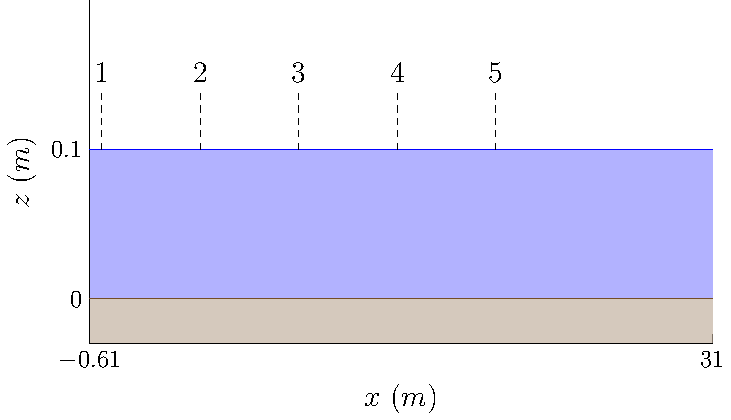
\includegraphics[width=\textwidth]{./chp6/figures/Experiment/Segur/WaveTank.pdf}
	\caption{Diagram demonstrating the water (\squareF{blue}) and the bed (\squareF{brown!80!black}) for the Segur experiments, with the wave gauge locations marked.}
	\label{fig:SegurWT}
\end{figure}

\subsection{Results for $0.01m$ Rectangular Depression}

Plots comparing the numerical and experimental wave gauge data for the $0.01m$ rectangular depression are displayed in Figures \ref{fig:Segur1cmFEVM} and \ref{fig:Segur1cmFDVM} for $\text{FEVM}_2$ and $\text{FDVM}_2$ respectively. Tables \ref{tab:ConservationSegurFEVM1cm} and \ref{tab:ConservationSegurFDVM1cm} are also provided, which record the conservation of all the quantities. 

The methods both produce results that overall agree well with the experimental results; particularly the initial triangular wave and the front of the dispersive wave train. While all the conserved quantities have indeed been conserved very well by the methods.  

The numerical solutions produce larger and consequently faster waves and observe oscillations in the depression which are not observed in the experimental data of wave gauge $1$. As expected the methods produce many more oscillations than were observed experimentally. These discrepancies can be attributed to the lack of viscosity and friction in the Serre equations \eqref{eqn:FullSerreCon}. Also most likely the experiment did not produce a discontinuous jump in the water depth with the downstroke of the piston which can significantly attenuate the higher frequency waves in the generated dispersive wavetrain \cite{Pitt-2018-61}. Given these limitations the numerical methods do a very good job of replicating the experimental behaviour. 

Both $\text{FEVM}_2$ and $\text{FDVM}_2$ have produced visually identical results at this scale and have demonstrated very good conservation of all the quantities in Tables \ref{tab:ConservationSegurFEVM1cm} and \ref{tab:ConservationSegurFDVM1cm}. Given the extensive review of these methods \cite{Pitt-2018-61} for steep gradient problems, this indicates that these solutions are indicative of true solutions of the Serre equations.
%Par 1: Figures

%Par 2: Discussion
	%phase and amplitude different (larger waves move faster)
	%waves on downstroke not present, suggesting that either gradient of down stroke not as steep, or waves are diffused stronger in thge real world
	%capture overall behaviour very well

%Par 3: Conclusion

%\ref{fig:Segur1cmFEVM} \ref{fig:Segur1cmFDVM}


\begin{figure}
	\centering
	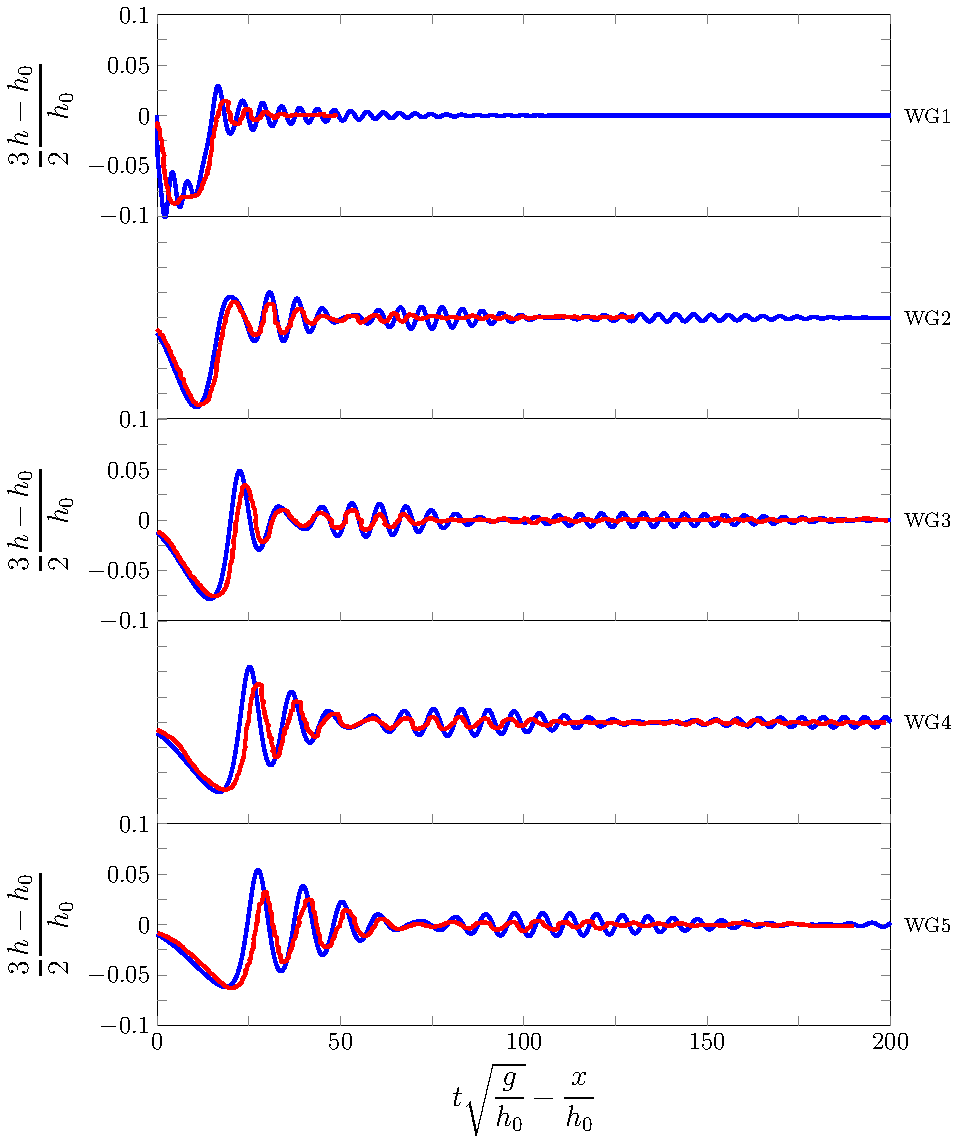
\includegraphics[width=\textwidth]{./chp6/figures/Experiment/Segur/LongWGsFEVM1cm.pdf}
	\caption{FEVM}
	\label{fig:Segur1cmFEVM}
\end{figure}
\begin{figure}
	\centering
	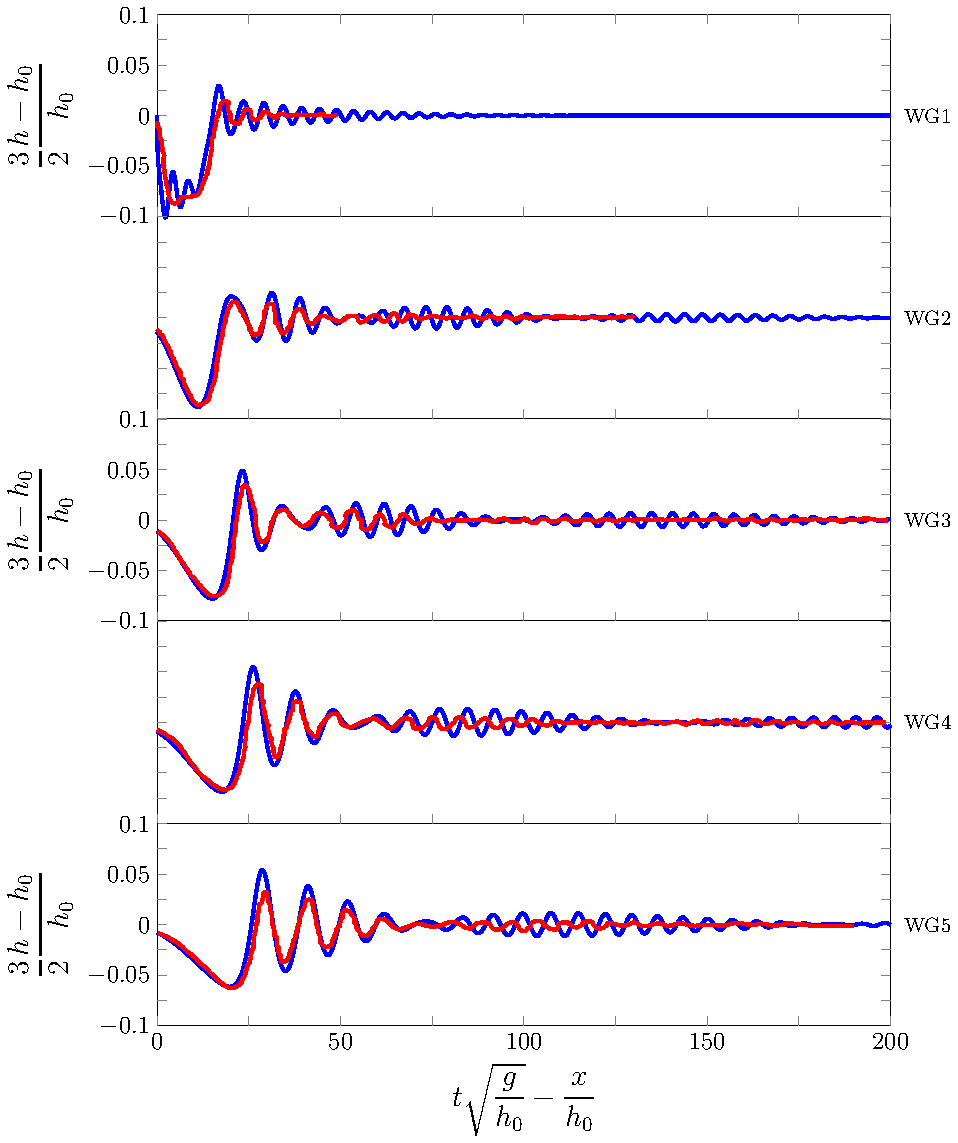
\includegraphics[width=\textwidth]{./chp6/figures/Experiment/Segur/LongWGsFDVM1cm.pdf}
	\caption{FDVM}
	\label{fig:Segur1cmFDVM}
\end{figure} 

\begin{table}
	\centering
	\begin{tabular}{l  c  c c}
		Quantity& $\mathcal{C}^*\left(\vecn{q}^0\right)$ & $\mathcal{C}^*\left(\vecn{q}^*\right)$ & $\mathcal{C}^*_1\left(\vecn{q}^0,\vecn{q}^*\right)$ \\
		\hline &&& \\
		Mass & $11.9888$ & $11.9888$ & $0$\\
		Momentum & $0$ & $7.44 \times 10^{-18}$ & $7.44 \times 10^{-18}$\\
		$G$ & $0$ & $1.56\times 10^{-18}$ & $1.56\times 10^{-18}$\\
		Energy & $5.8751204081$ & $5.8750869556$ & $5.70 \times 10^{-6}$ \\
	\end{tabular}
	\caption{Total amounts and error in conservation for all quantities for $\text{FEVM}_2$ numerical solution of the $0.01m$ rectangular depression.}
	\label{tab:ConservationSegurFEVM1cm}
\end{table} 



\begin{table}
	\centering
	\begin{tabular}{l  c  c c}
		Quantity& $\mathcal{C}^*\left(\vecn{q}^0\right)$ & $\mathcal{C}^*\left(\vecn{q}^*\right)$ & $\mathcal{C}^*_1\left(\vecn{q}^0,\vecn{q}^*\right)$ \\
		\hline &&& \\
		Mass & $11.9888$ & $11.9888$ & $0$\\
		Momentum & $0$ & $-1.19 \times 10^{-17}$ & $-1.19 \times 10^{-17}$\\
		$G$ & $0$ & $-8.05\times 10^{-18}$ & $-8.05\times 10^{-18}$\\
		Energy & $5.8751204081$ & $5.87508358202$ & $6.27 \times 10^{-6}$ \\
	\end{tabular}
	\caption{Total amounts and error in conservation for all quantities for $\text{FDVM}_2$ numerical solution of the $0.01m$ rectangular depression.}
	\label{tab:ConservationSegurFDVM1cm}
\end{table}  
 

\subsection{Results for $0.03m$ Rectangular Depression}

The wave gauge data for the numerical and experimental results for the evolution of the $0.03m$ rectangular depression are displayed in Figures \ref{fig:Segur3cmFEVM} and \ref{fig:Segur3cmFDVM} for $\text{FEVM}_2$ and $\text{FDVM}_2$ respectively. The conservation of all the conserved quantities are given in Tables \ref{tab:ConservationSegurFEVM3cm} and \ref{tab:ConservationSegurFEVM3cm} for $\text{FEVM}_2$ and $\text{FDVM}_2$ respectively.

Both methods again reproduce the overall behaviour of this experiment very well. Because the rectangular wave is deeper, this experiment provides a more rigorous test for the numerical methods. However, because there is more energy and the piston has to move further to generate the wave the effects that damp the oscillations in the experiments are more significant leading to a much larger difference between the numerical and experimental results; particularly for the amplitude and speed of the waves.

Since the rectangular depression is larger the numerical methods have a larger error in conservation for all the quantities as compared to the $0.01m$ rectangular depression except mass; which is conserved exactly. For $G$ and momentum these errors are around machine epsilon and can be disregarded, so that only the conservation of energy is significantly effected. Even with this larger error, all quantities are still well conserved by the numerical methods, suggesting that our numerical solutions well represent the true solutions of the Serre equations. 

These experiments have been well replicated by the numerical methods, and given the resolution and error in conservation and the extensive study summarised in []; these results demonstrate that we are solving the Serre equations in the presence of steep gradients very well and that the behaviour of steep gradients in experiments aligns well with their behaviour in the Serre equations. 

%Par 1: Figures

%Par 2: Discussion
	%phase and amplitude different (larger waves move faster)
	%waves on downstroke not present, suggesting that either gradient of down stroke not as steep, or waves are diffused stronger in thge real world
	%capture overall behaviour very well

%Par 3: Conclusion

%\ref{fig:Segur3cmFEVM} \ref{fig:Segur3cmFDVM}
     
\begin{figure}
	\centering
	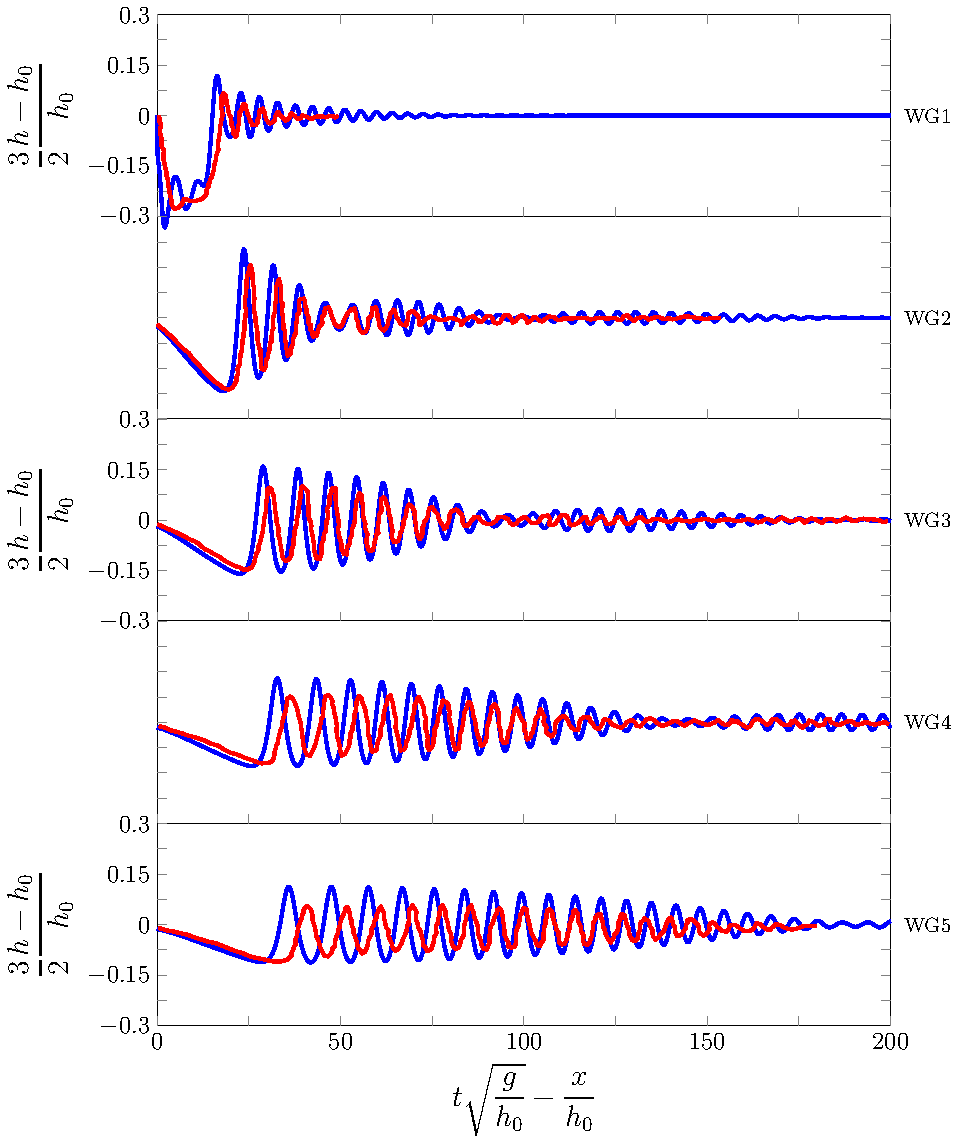
\includegraphics[width=\textwidth]{./chp6/figures/Experiment/Segur/LongWGsFEVM3cm.pdf}
	\caption{FEVM}
	\label{fig:Segur3cmFEVM}
\end{figure}
\begin{figure}
	\centering
	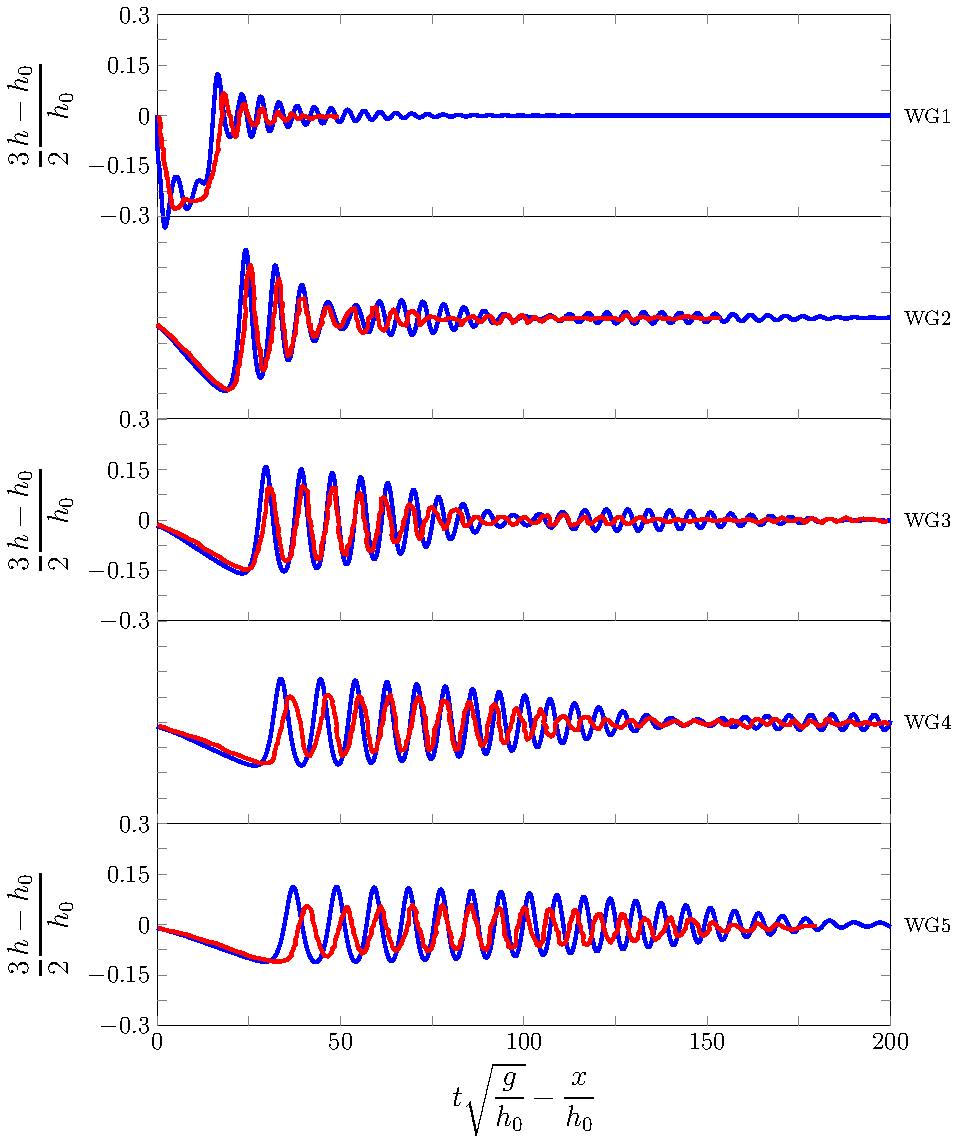
\includegraphics[width=\textwidth]{./chp6/figures/Experiment/Segur/LongWGsFDVM3cm.pdf}
	\caption{FDVM}
	\label{fig:Segur3cmFDVM}
\end{figure}  

\begin{table}
	\centering
	\begin{tabular}{l  c  c c}
		Quantity& $\mathcal{C}^*\left(\vecn{q}^0\right)$ & $\mathcal{C}^*\left(\vecn{q}^*\right)$ & $\mathcal{C}^*_1\left(\vecn{q}^0,\vecn{q}^*\right)$ \\
		\hline &&& \\
		Mass & $11.9644$ & $11.9644$ & $0$\\
		Momentum & $0$ & $-7.75 \times 10^{-17}$ & $-7.75\times 10^{-17}$\\
		$G$ & $0$ & $-3.33\times 10^{-16}$ & $-3.33\times 10^{-16}$\\
		Energy & $5.85596887293$ & $5.85524264766 $ & $1.24 \times 10^{-4}$ \\
	\end{tabular}
	\caption{Total amounts and error in conservation for all quantities for $\text{FEVM}_2$ numerical solution of the $0.03m$ rectangular depression.}
	\label{tab:ConservationSegurFEVM3cm}
\end{table} 



\begin{table}
	\centering
	\begin{tabular}{l  c  c c}
		Quantity& $\mathcal{C}^*\left(\vecn{q}^0\right)$ & $\mathcal{C}^*\left(\vecn{q}^*\right)$ & $\mathcal{C}^*_1\left(\vecn{q}^0,\vecn{q}^*\right)$ \\
		\hline &&& \\
		Mass & $11.9644$ & $11.9644$ & $0$\\
		Momentum & $0$ & $-9.09 \times 10^{-17}$ & $-9.09 \times 10^{-17}$\\
		$G$ & $0$ & $-1.16\times 10^{-16}$ & $-1.16\times 10^{-16}$\\
		Energy & $5.85596887293$ & $5.85520859829 $ & $1.30 \times 10^{-4}$ \\
	\end{tabular}
	\caption{Total amounts and error in conservation for all quantities for $\text{FDVM}_2$ numerical solution of the $0.03m$ rectangular depression.}
	\label{tab:ConservationSegurFDVM3cm}
\end{table}  


\section{Periodic Waves Over A Submerged Bar}
\label{sec:PeriodicWavessubBar}
%only pointwise comparison
Beji and Battjes conducted a series of experiments investigating the effect of submerged bars on the propagation of periodic waves \cite{Beji-Battjes-1993-151,Beji-Battjes-1994-1}. The behaviour of these experiments were mainly driven by the dispersion properties of the waves and their interaction with variations in bathymetry. Therefore, these experiments serve as a good benchmark for our numerical schemes abilities to accurately model both the effect of variable bathymetry and dispersive waves. For our purposes we will focus on the monochromatic wave experiments of \citet{Beji-Battjes-1994-1}.

The experiments of \citet{Beji-Battjes-1994-1} were conducted in a wave tank $37.7m$ long, $0.8m$ wide and $0.75m$ high. A diagram of the longitudinal section of the wave tank is given in Figure \ref{fig:BejiWT}. There are seven wave gauges at the following locations; $5.7m$, $10.5m$, $12.5m$, $13.5m$, $14.5m$, $15.7m$ and $17.3m$. Waves are generated from a piston-type wave maker located at $0m$ and travel on the initially still water to the right, over the submerged trapezoidal bar towards a wave absorbing sloped beach.

Two sinusoidal monochromatic non-breaking wave experiments were conducted. A low frequency one with a wavelength $\lambda \approx 3.69m$ and a period of $T = 2s$, and a high frequency one with $\lambda \approx 2.05m$ and a period of $T = 1.25s$. Both experiments had a wave amplitude of $0.01m$ and so both had the same non-linearity parameter $\epsilon = 0.01 / 0.4 = 0.025$. 

We numerically simulated these experiments over the spatial domain $\left[5.7m,150m\right]$ with $\Delta x = 0.1 / 2^4 m$ and $\Delta t = Sp / 2^5$ where $Sp = 0.039$ is the experimental sampling period. These $\Delta x$ and $\Delta t$ values satisfy the CFL condition \eqref{eqn:CFLcond} for these experiments. In our numerical experiments only the submerged trapezoidal bar is present, and the sloping beach is replaced with a very long horizontal bed that ensures that we do not observe any boundary effects in our results.  

To simulate the incoming waves at the upstream boundary we used the first wave gauge as our left boundary condition and used linear extrapolation to calculate the other required $h$ values in the left ghost cell. The velocity boundary conditions were calculated from the height values by solving the continuity equation \eqref{eqn:FullSerreNonConMass} assuming $u$ and $h$ are travelling wave solutions
\begin{equation*}
u(x,t) = \sqrt{g h_0} \; \dfrac{h(x,t) - h_0}{h(x,t)}.
\end{equation*}
Finally the boundary conditions for $G$ were calculated using the boundary conditions for $h$ and $u$. We shall now present our numerical results for the low and high frequency experiments.
%
\begin{figure}
	\centering
		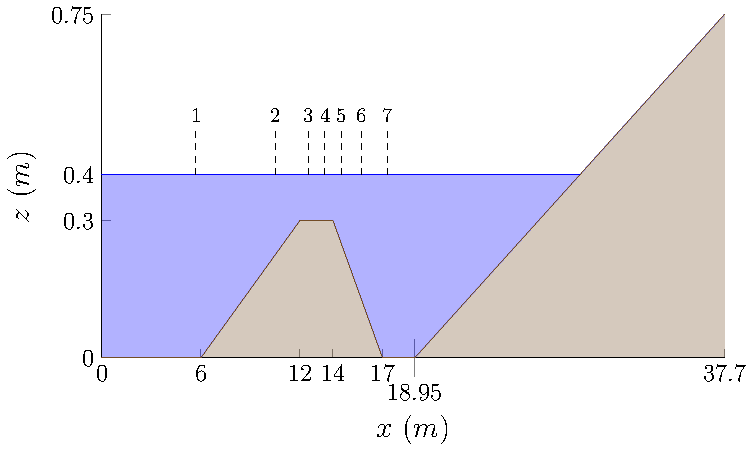
\includegraphics[width=\textwidth]{./chp6/figures/Experiment/Beji/BejiTank.pdf}
	\caption{Diagram demonstrating the water (\squareF{blue}) and the ground  (\squareF{brown!80!black}) for the Beji experiments, with the wave gauge locations marked.}
	\label{fig:BejiWT}
\end{figure}
%
\subsection{Low Frequency Results}
A comparison of wave heights of the experimental and numerical results are located in Figures \ref{fig:BejislWG1to4FEVM} and \ref{fig:BejislWG5to7FEVM} for $\text{FEVM}_2$ and Figures \ref{fig:BejislWG1to4FDVM} and \ref{fig:BejislWG5to7FDVM} for $\text{FDVM}_2$. These numerical schemes both produce identical results for all wave gauges and so this benchmark does not help us discriminate between these two methods. 

These results demonstrate the ability of these numerical methods to recreate the experimental results, particularly for wave gauge $1$ to $5$ where the agreement between experimental and numerical results is best. This validates the numerical schemes for simulating shoaling of dispersion waves as these wave gauges are all located on the windward side of the submerged bar where shoaling occurs in the experiment. 

The numerical results for wave gauges $6$ and $7$ on the leeward side capture some of the wave behaviour but their agreement with the experiments results is much worse. The inadequacy of the numerical results here appears to be due to the discrepancy between the dispersion properties of the Serre equations and water waves, as the numerical solutions of improved dispersion equations \cite{Beji-Battjes-1994-1,Lannes-2013} accurately reproduce the experimental results on the leeward side.

The dispersion of the Serre equations is vital to recreating the experimental results for wave gauges $2$ to $5$, as non-dispersive equations such as the SWWE do a very poor job at simulating this experiment \cite{Pitt-2017-1725}. However, to properly reproduce the experimental results on the leeward side of the slope at wave gauges $6$ and $7$  would require improving the dispersion characteristics of the underlying Serre equations as done by \citet{Barthelemy-2004-315}. Such an improvement can be incorporated into the hybrid FDVM and FEVM numerical methods \cite{Zoppou-2014} but is beyond the scope of this thesis. 

\begin{figure}
	\centering
	\begin{subfigure}{0.5\textwidth}
		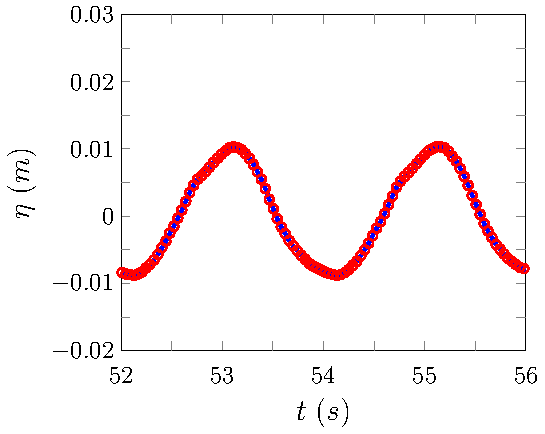
\includegraphics[width=\textwidth]{./chp6/figures/Experiment/Beji/sl/FEVMWG1.pdf}
		\subcaption{Wave Gauge $1$}
		\vspace{0.5cm}
	\end{subfigure}%
	\begin{subfigure}{0.5\textwidth}
		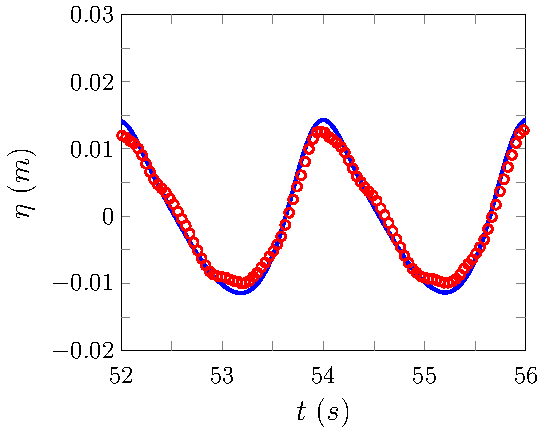
\includegraphics[width=\textwidth]{./chp6/figures/Experiment/Beji/sl/FEVMWG2.pdf}
		\subcaption{Wave Gauge $2$}
		\vspace{0.5cm}
	\end{subfigure}
	\begin{subfigure}{0.5\textwidth}
		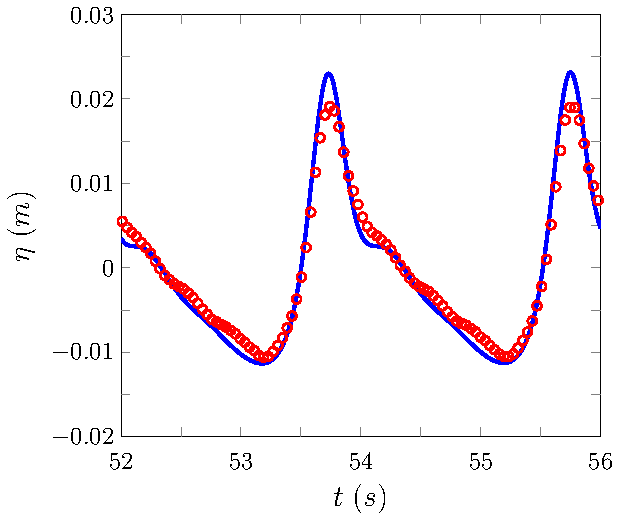
\includegraphics[width=\textwidth]{./chp6/figures/Experiment/Beji/sl/FEVMWG3.pdf}
		\subcaption{Wave Gauge $3$}
		\vspace{0.5cm}
	\end{subfigure}%
	\begin{subfigure}{0.5\textwidth}
		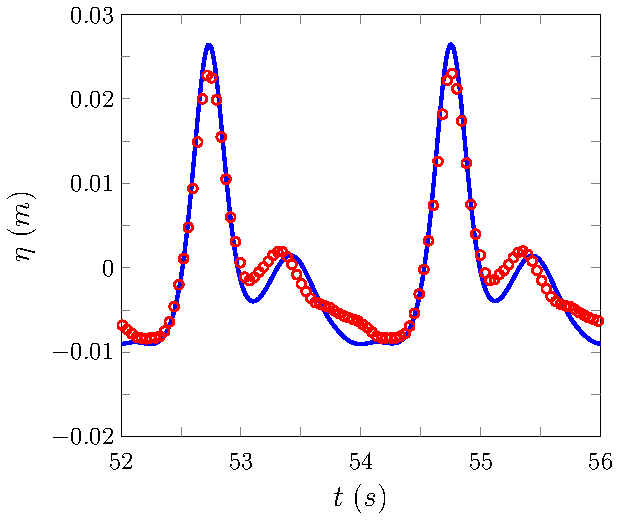
\includegraphics[width=\textwidth]{./chp6/figures/Experiment/Beji/sl/FEVMWG4.pdf}
		\subcaption{Wave Gauge $4$}
		\vspace{0.5cm}
	\end{subfigure}
	\caption{Comparison of the wave heights $\eta$ of the numerical results for the $\text{FEVM}_2$ ({\color{blue}\solidrule}) and the experimental results (\circlet{red}) for wave gauges $1$ - $4$ for the low frequency experiment.}
	\label{fig:BejislWG1to4FEVM}
\end{figure}

\begin{figure}
	\centering
	\begin{subfigure}{0.5\textwidth}
		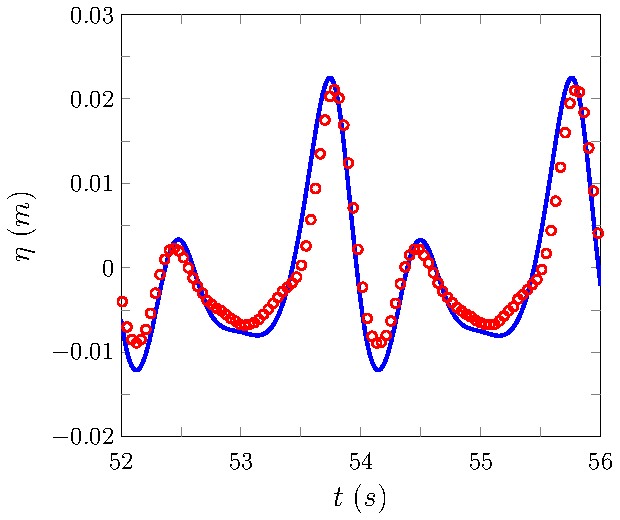
\includegraphics[width=\textwidth]{./chp6/figures/Experiment/Beji/sl/FEVMWG5.pdf}
		\subcaption{Wave Gauge $5$}
		\vspace{0.5cm}
	\end{subfigure}%
	\begin{subfigure}{0.5\textwidth}
		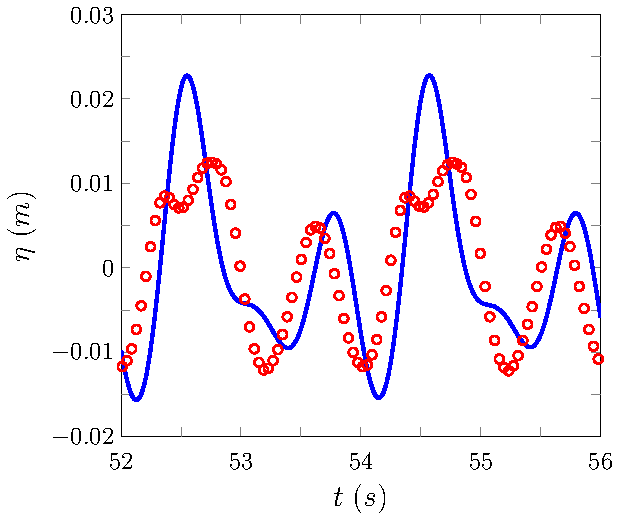
\includegraphics[width=\textwidth]{./chp6/figures/Experiment/Beji/sl/FEVMWG6.pdf}
		\subcaption{Wave Gauge $6$}
		\vspace{0.5cm}
	\end{subfigure}
	\begin{subfigure}{0.5\textwidth}
		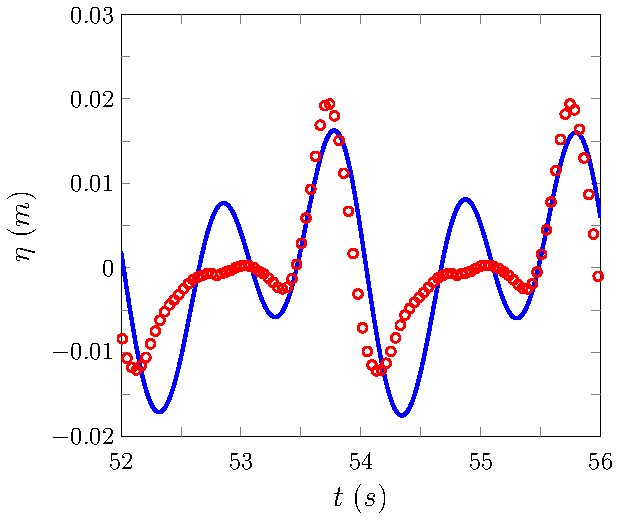
\includegraphics[width=\textwidth]{./chp6/figures/Experiment/Beji/sl/FEVMWG7.pdf}
		\subcaption{Wave Gauge $7$}
		\vspace{0.5cm}
	\end{subfigure}
	\caption{Comparison of the wave heights $\eta$ of the numerical results for the $\text{FEVM}_2$ ({\color{blue}\solidrule}) and the experimental results (\circlet{red}) for wave gauges $5$ - $7$ for the low frequency experiment.}
	\label{fig:BejislWG5to7FEVM}
\end{figure}


\begin{figure}
	\centering
	\begin{subfigure}{0.5\textwidth}
		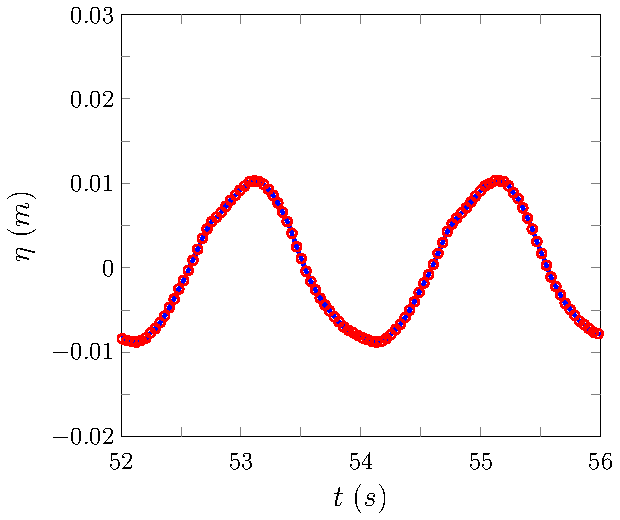
\includegraphics[width=\textwidth]{./chp6/figures/Experiment/Beji/sl/FDVMWG1.pdf}
		\subcaption{Wave Gauge $1$}
		\vspace{0.5cm}
	\end{subfigure}%
	\begin{subfigure}{0.5\textwidth}
		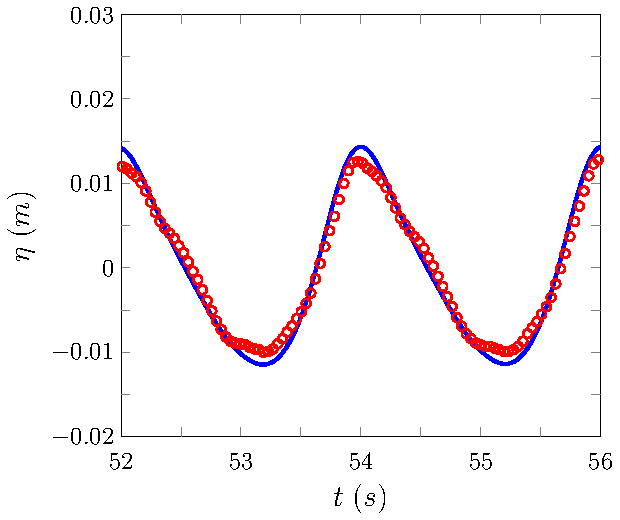
\includegraphics[width=\textwidth]{./chp6/figures/Experiment/Beji/sl/FDVMWG2.pdf}
		\subcaption{Wave Gauge $2$}
		\vspace{0.5cm}
	\end{subfigure}
	\begin{subfigure}{0.5\textwidth}
		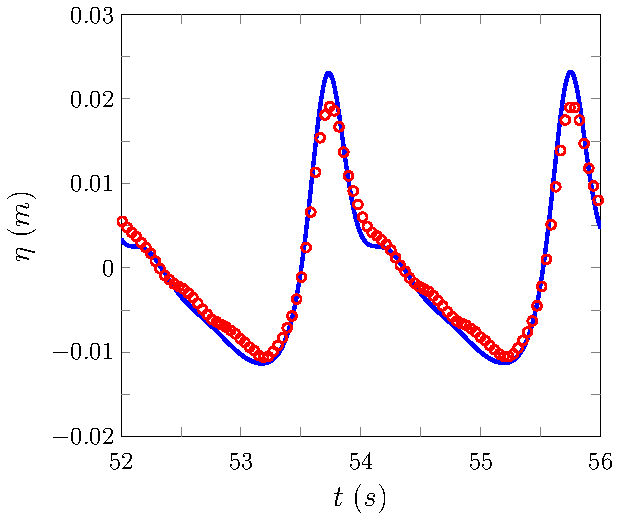
\includegraphics[width=\textwidth]{./chp6/figures/Experiment/Beji/sl/FDVMWG3.pdf}
		\subcaption{Wave Gauge $3$}
		\vspace{0.5cm}
	\end{subfigure}%
	\begin{subfigure}{0.5\textwidth}
		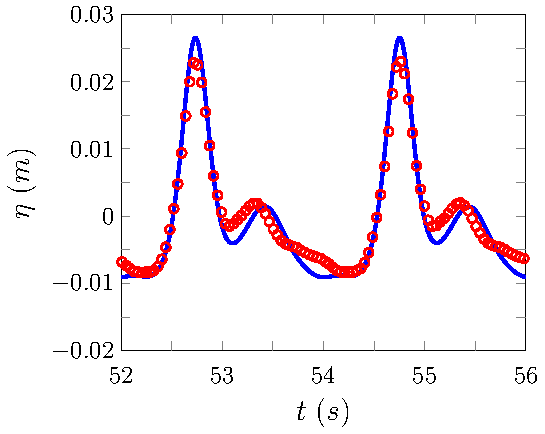
\includegraphics[width=\textwidth]{./chp6/figures/Experiment/Beji/sl/FDVMWG4.pdf}
		\subcaption{Wave Gauge $4$}
		\vspace{0.5cm}
	\end{subfigure}
	\caption{Comparison of the wave heights $\eta$ of the numerical results for the $\text{FDVM}_2$ ({\color{blue}\solidrule}) and the experimental results (\circlet{red}) for wave gauges $1$ - $4$ for the low frequency experiment.}
	\label{fig:BejislWG1to4FDVM}
\end{figure}

\begin{figure}
	\centering
	\begin{subfigure}{0.5\textwidth}
		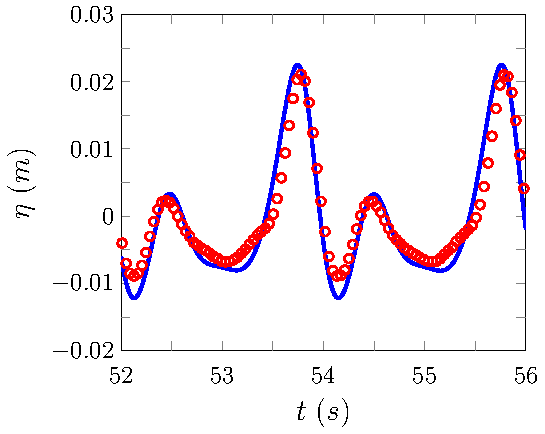
\includegraphics[width=\textwidth]{./chp6/figures/Experiment/Beji/sl/FDVMWG5.pdf}
		\subcaption{Wave Gauge $5$}
		\vspace{0.5cm}
	\end{subfigure}%
	\begin{subfigure}{0.5\textwidth}
		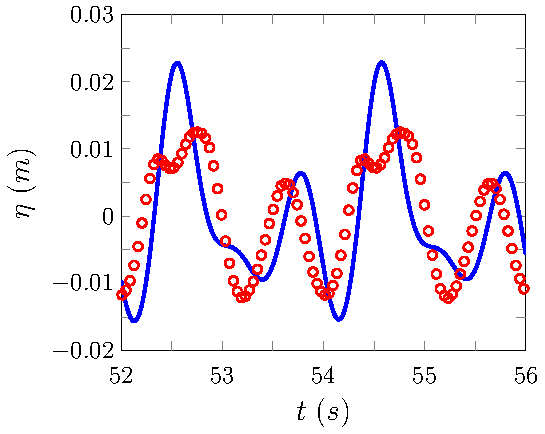
\includegraphics[width=\textwidth]{./chp6/figures/Experiment/Beji/sl/FDVMWG6.pdf}
		\subcaption{Wave Gauge $6$}
		\vspace{0.5cm}
	\end{subfigure}
	\begin{subfigure}{0.5\textwidth}
		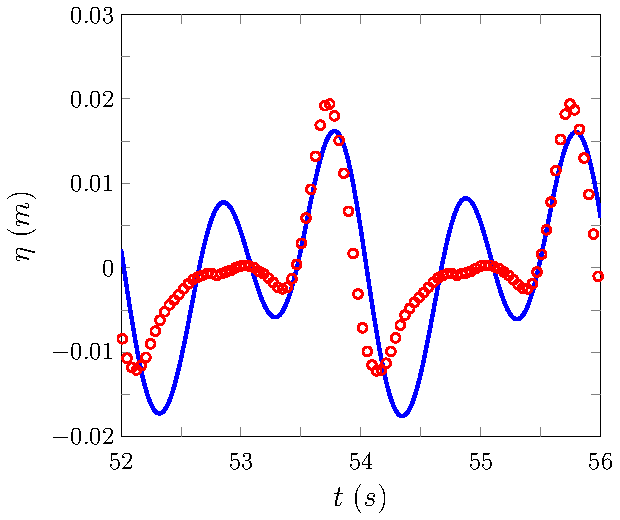
\includegraphics[width=\textwidth]{./chp6/figures/Experiment/Beji/sl/FDVMWG7.pdf}
		\subcaption{Wave Gauge $7$}
		\vspace{0.5cm}
	\end{subfigure}
	\caption{Comparison of the wave heights $\eta$ of the numerical results for the $\text{FDVM}_2$ ({\color{blue}\solidrule}) and the experimental results (\circlet{red}) for wave gauges $5$ - $7$ for the low frequency experiment.}
	\label{fig:BejislWG5to7FDVM}
\end{figure}

\subsection{High Frequency Results}
The wave heights of the experimental and numerical results are given in Figures \ref{fig:BejishWG1to4FEVM} and \ref{fig:BejishWG5to7FEVM} for $\text{FEVM}_2$. While the results for $\text{FDVM}_2$ are given in Figures \ref{fig:BejishWG1to4FDVM} and \ref{fig:BejishWG5to7FDVM}. As for the low frequency experiment, these numerical schemes $\text{FEVM}_2$ and $\text{FDVM}_2$ produce identical results for all wave gauges at this scale and so this benchmark does not discriminate between these two methods. 

As in the low frequency experiment we observe that the numerical results perform well on the windward side of the slope for wave gauges $1$ to $4$ but perform poorly for the leeward side of the slope for wave gauges $5$ to $7$. With the high frequency experiment we see the divergence between the numerical and experimental results earlier than the low frequency experiment, so that now wave gauge 5 which is on the leeward side exhibits a significant difference between the numerical and experimental results. As in the low frequency example improving the dispersion properties of the governing partial differential equations lead to a much better agreement between the numerical and experimental results \cite{Beji-Battjes-1994-1,Lannes-2013}. Because the difference between the dispersion relation of the Serre equations and water waves is largest for higher frequency and therefore for shorter waves \citet{Barthelemy-2004-315} the earlier divergence between experimental and numerical results is expected. 

These numerical results for the $\text{FDVM}_2$ and $\text{FEVM}_2$ agree well with other numerical results for weakly dispersive equations without improved dispersion properties for the simulation of periodic waves over a submerged bar in the literature \cite{Beji-Battjes-1994-1,Lannes-2013,Li-2014-169,Zhang-2013-13}. Therefore, without changing the underlying partial differential equations, our numerical methods perform as numerical schemes in the literature at recreating the experimental results of \citet{Beji-Battjes-1994-1}.

\begin{figure}
	\centering
	\begin{subfigure}{0.5\textwidth}
		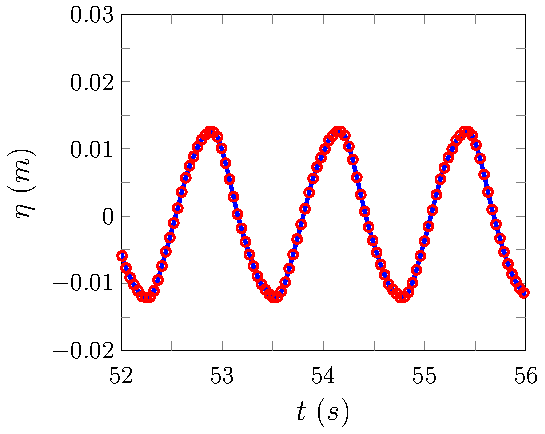
\includegraphics[width=\textwidth]{./chp6/figures/Experiment/Beji/sh/FEVMWG1.pdf}
		\subcaption{Wave Gauge $1$}
		\vspace{0.5cm}
	\end{subfigure}%
	\begin{subfigure}{0.5\textwidth}
		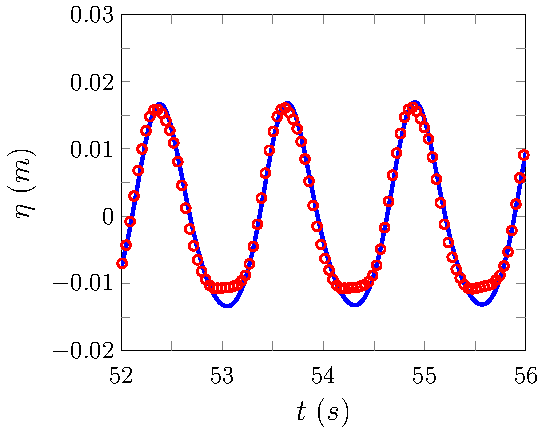
\includegraphics[width=\textwidth]{./chp6/figures/Experiment/Beji/sh/FEVMWG2.pdf}
		\subcaption{Wave Gauge $2$}
		\vspace{0.5cm}
	\end{subfigure}
	\begin{subfigure}{0.5\textwidth}
		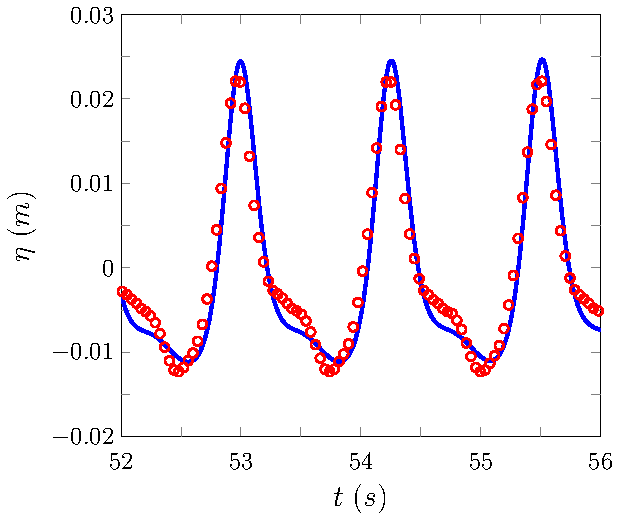
\includegraphics[width=\textwidth]{./chp6/figures/Experiment/Beji/sh/FEVMWG3.pdf}
		\subcaption{Wave Gauge $3$}
		\vspace{0.5cm}
	\end{subfigure}%
	\begin{subfigure}{0.5\textwidth}
		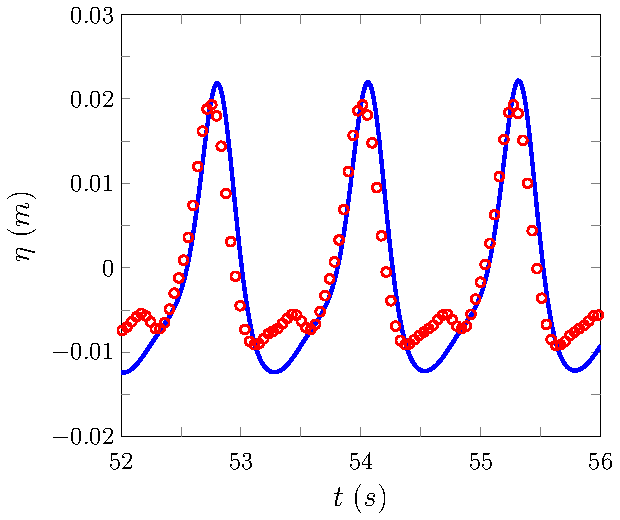
\includegraphics[width=\textwidth]{./chp6/figures/Experiment/Beji/sh/FEVMWG4.pdf}
		\subcaption{Wave Gauge $4$}
		\vspace{0.5cm}
	\end{subfigure}
	\caption{Comparison of the wave heights $\eta$ of the numerical results for the $\text{FEVM}_2$ ({\color{blue}\solidrule}) and the experimental results (\circlet{red}) for wave gauges $1$ - $4$ for the low frequency experiment.}
	\label{fig:BejishWG1to4FEVM}
\end{figure}

\begin{figure}
	\centering
	\begin{subfigure}{0.5\textwidth}
		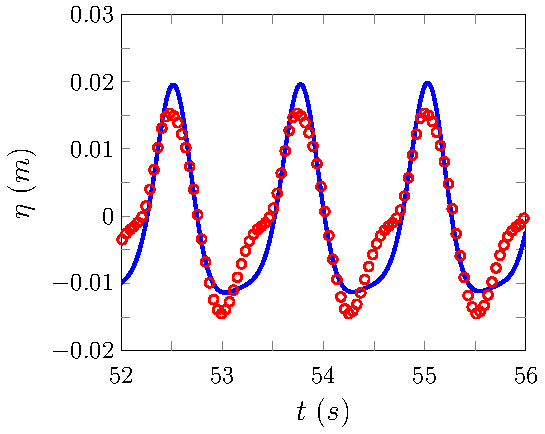
\includegraphics[width=\textwidth]{./chp6/figures/Experiment/Beji/sh/FEVMWG5.pdf}
		\subcaption{Wave Gauge $5$}
		\vspace{0.5cm}
	\end{subfigure}%
	\begin{subfigure}{0.5\textwidth}
		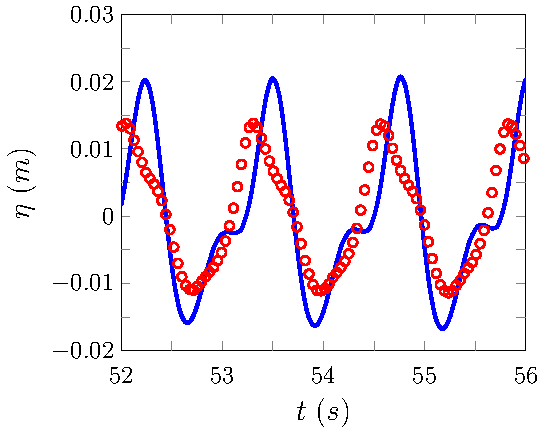
\includegraphics[width=\textwidth]{./chp6/figures/Experiment/Beji/sh/FEVMWG6.pdf}
		\subcaption{Wave Gauge $6$}
		\vspace{0.5cm}
	\end{subfigure}
	\begin{subfigure}{0.5\textwidth}
		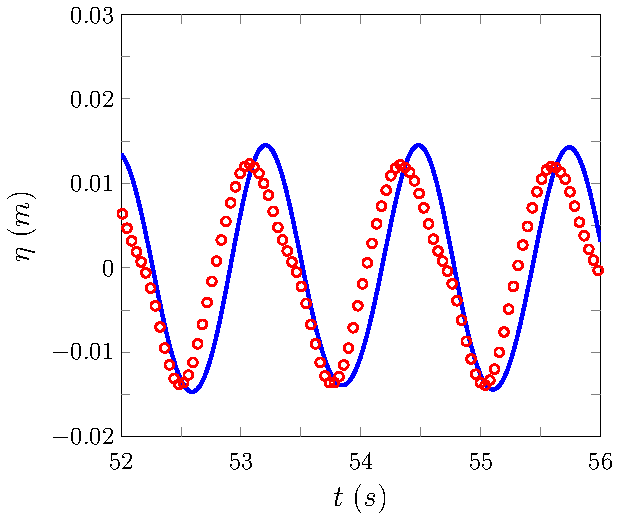
\includegraphics[width=\textwidth]{./chp6/figures/Experiment/Beji/sh/FEVMWG7.pdf}
		\subcaption{Wave Gauge $7$}
		\vspace{0.5cm}
	\end{subfigure}
	\caption{Comparison of the wave heights $\eta$ of the numerical results for the $\text{FEVM}_2$ ({\color{blue}\solidrule}) and the experimental results (\circlet{red}) for wave gauges $5$ - $7$ for the high frequency experiment.}
	\label{fig:BejishWG5to7FEVM}
\end{figure}


\begin{figure}
	\centering
	\begin{subfigure}{0.5\textwidth}
		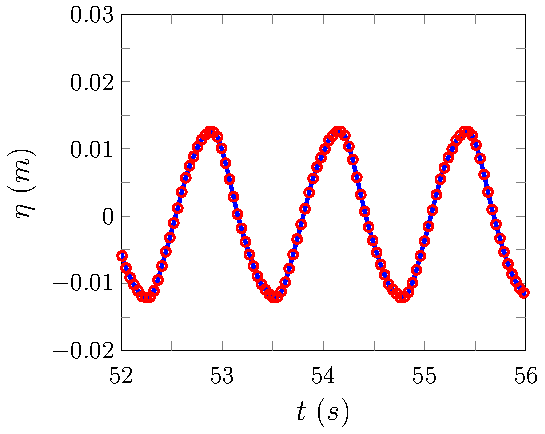
\includegraphics[width=\textwidth]{./chp6/figures/Experiment/Beji/sh/FDVMWG1.pdf}
		\subcaption{Wave Gauge $1$}
		\vspace{0.5cm}
	\end{subfigure}%
	\begin{subfigure}{0.5\textwidth}
		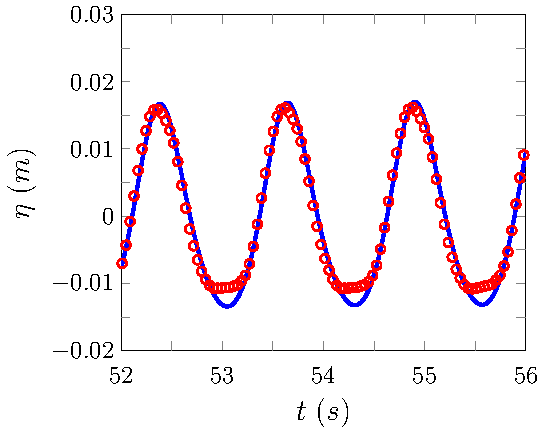
\includegraphics[width=\textwidth]{./chp6/figures/Experiment/Beji/sh/FDVMWG2.pdf}
		\subcaption{Wave Gauge $2$}
		\vspace{0.5cm}
	\end{subfigure}
	\begin{subfigure}{0.5\textwidth}
		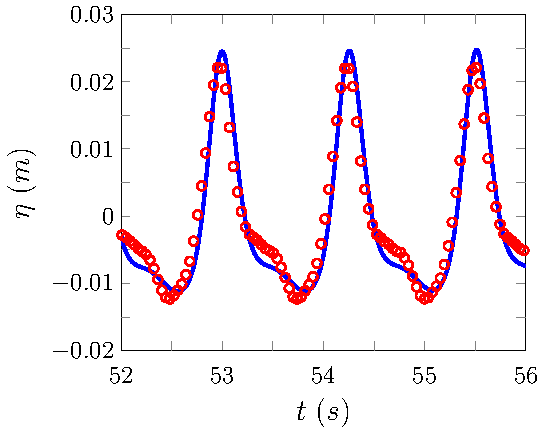
\includegraphics[width=\textwidth]{./chp6/figures/Experiment/Beji/sh/FDVMWG3.pdf}
		\subcaption{Wave Gauge $3$}
		\vspace{0.5cm}
	\end{subfigure}%
	\begin{subfigure}{0.5\textwidth}
		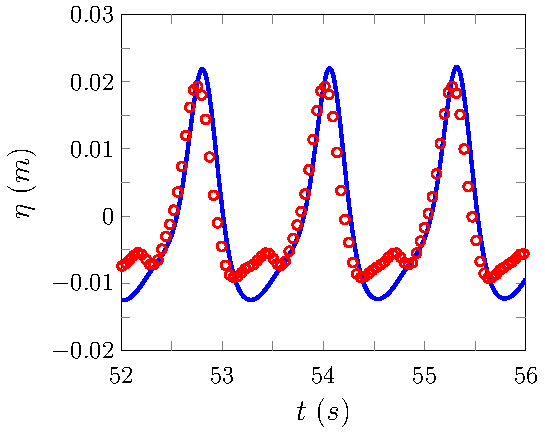
\includegraphics[width=\textwidth]{./chp6/figures/Experiment/Beji/sh/FDVMWG4.pdf}
		\subcaption{Wave Gauge $4$}
		\vspace{0.5cm}
	\end{subfigure}
	\caption{Comparison of the wave heights $\eta$ of the numerical results for the $\text{FDVM}_2$ ({\color{blue}\solidrule}) and the experimental results (\circlet{red}) for wave gauges $1$ - $4$ for the high frequency experiment.}
	\label{fig:BejishWG1to4FDVM}
\end{figure}

\begin{figure}
	\centering
	\begin{subfigure}{0.5\textwidth}
		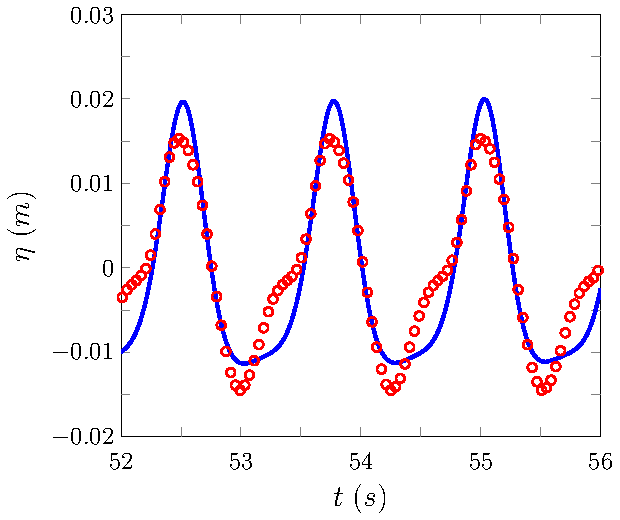
\includegraphics[width=\textwidth]{./chp6/figures/Experiment/Beji/sh/FDVMWG5.pdf}
		\subcaption{Wave Gauge $5$}
		\vspace{0.5cm}
	\end{subfigure}%
	\begin{subfigure}{0.5\textwidth}
		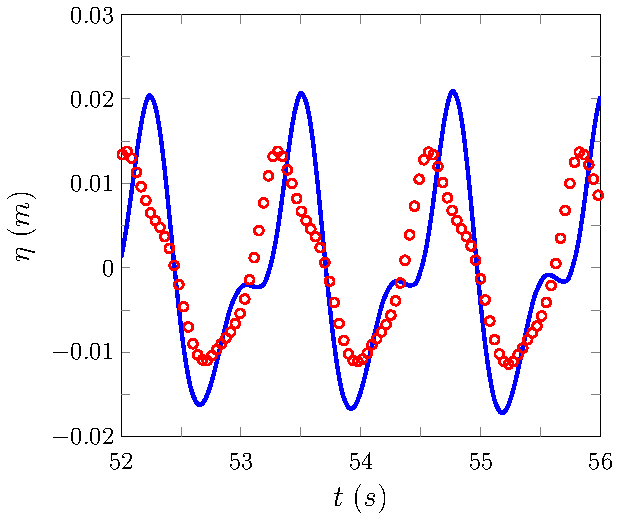
\includegraphics[width=\textwidth]{./chp6/figures/Experiment/Beji/sh/FDVMWG6.pdf}
		\subcaption{Wave Gauge $6$}
		\vspace{0.5cm}
	\end{subfigure}
	\begin{subfigure}{0.5\textwidth}
		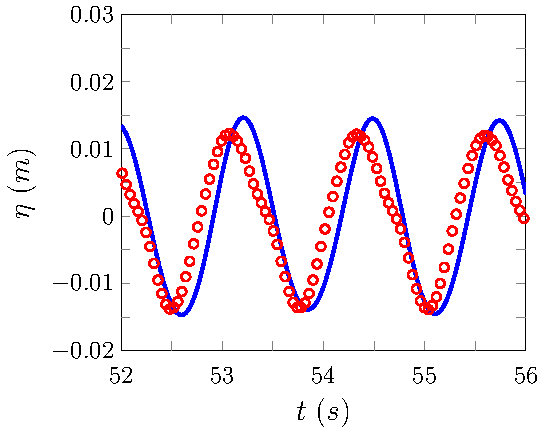
\includegraphics[width=\textwidth]{./chp6/figures/Experiment/Beji/sh/FDVMWG7.pdf}
		\subcaption{Wave Gauge $7$}
		\vspace{0.5cm}
	\end{subfigure}
	\caption{Comparison of the wave heights $\eta$ of the numerical results for the $\text{FDVM}_2$ ({\color{blue}\solidrule}) and the experimental results (\circlet{red}) for wave gauges $5$ - $7$ for the high frequency experiment.}
	\label{fig:BejishWG5to7FDVM}
\end{figure}

\section{Roeber}
%Wave gauge
%way beyond nolinearity paramter
%in fact this wave breaks, leading to large air entrainment

%wave breaking
%>>> 66 / (sqrt(9.81/2.46))
%33.050420197470373
%>>> 64 / (sqrt(9.81/2.46))
%32.048892312698548

%friction damps these trialing waves?

%comment on wave breaking number for nonlinearity


%Fillipine/Roeber also show discrepancy between numerical model and data before the appearance of the reflected waves, assumption about them having the nolinearity speed may be dubious, good agreement with leading wave


%Par 1: Experimental Design
	%breaking wave on a fringing reef (check)

%Par 2: Explanation of Experiment and what it demonstrates
	%can compare the behaviour of dispersion and shaoling
	%can compare to other dispersive models (Roebers)

%Par 3: Numerical Experiment Design


To study the evolution of waves on fringing reefs a series of experiments were conducted by \citet{Roeber-2010}. These experiments were performed in a wave tank $3.66m$ wide, $83.7m$ long and $4.57m$ high with removable beds that allowed for the wide range of experiments reported by \citet{Roeber-2010}. We have computationally modelled the experiment with the bathymetry displayed in Figure \ref{fig:RoeberWT}, where a solitary wave is generated from the wavemaker at $0m$ and is recorded at the wave gauges at $17.6m$, $28.6m$, $35.9m$, $40.6m$, $44.3m$, $46.1m$, $48.2m$, $50.4m$, $54.4m$, $58.0m$, $61.7m$, $65.4m$, $72.7m$ and $80.0m$.

This experiment investigates the behaviour of waves with high nonlinearity $ \epsilon \approx 1.23/2.46 = 0.5$ as it shoals over a linear bed into a very thin body of water. Given the high nonlinearity of this wave, it is not surprising that as it shoals it becomes a plunging breaker which formed at $t \approx 32s$ with an elliptical air cavity observed at $t \approx 33s$. As with other depth averaged equations, the Serre equations cannot naively model breaking waves so this experiment is not an entirely appropriate test of the numerical methods, particularly after $32s$.

This experiment was numerically modelled on the domain $[17.6m , 400m]$ and was run until $t = 60s$ after which the reflections from the downstream end of the tank become significant in the experiment. The beginning of the domain was chosen so that wave gauge $1$ could be used as the left boundary conditions, where the technique in section \ref{sec:PeriodicWavessubBar} was employed. The spatial resolution was $\Delta x = 0.025m$ and the temporal resolution was $\Delta t = Sp / 8 s$ where $Sp = 0.02$ was the sampling period of the wave gauges, which satisfy the CFL condition \eqref{eqn:CFLcond}. The right edge of the domain used Dirichlet boundary conditions and no effects from the boundary conditions were observed in the numerical results. 



\begin{figure}
	\centering
	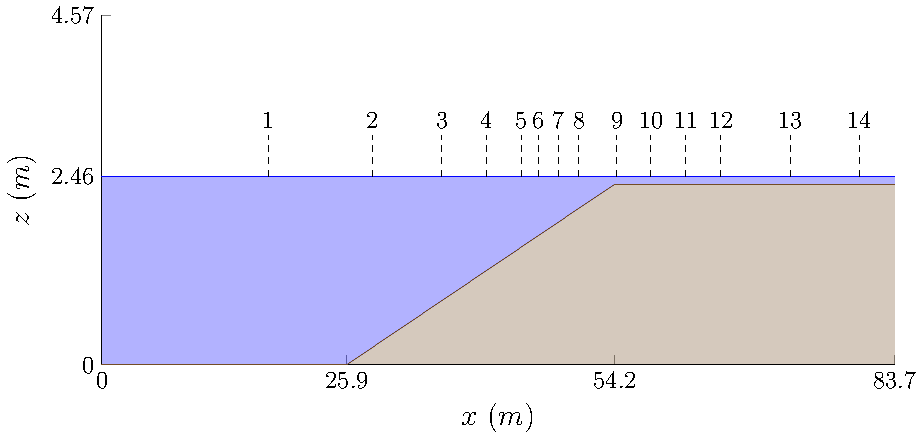
\includegraphics[width=\textwidth]{./chp6/figures/Experiment/Roeber/Trial8/WaveTank.pdf}
	\caption{Diagram demonstrating the water (\squareF{blue}) and the ground  (\squareF{brown!80!black}) for the Beji experiments, with the wave gauge locations marked.}
	\label{fig:RoeberWT}
\end{figure}

\subsection{Results}

The wave gauge results comparing the numerical and experimental data are displayed in Figures \ref{fig:Roeber8WG1to7FDVM} and \ref{fig:Roeber8WG7to14FDVM} for $\text{FDVM}_2$ and \ref{fig:Roeber8WG1to7FEVM} and \ref{fig:Roeber8WG7to14FEVM} for $\text{FEVM}_2$.

Both methods accurately reproduce the shoaling of the solitary wave, particularly in wave gauges $1$ through $8$ which record the wave before breaking begins. The behaviour of the trailing waves is not as well replicated, with the numerical solutions over predicting their amplitude and speed as  observed in the previous experiments.The reflected wave can also be observed in the wave gauges and since the numerical simulation did not have reflective boundaries these waves are not replicated in their solution.

When breaking begins as expected the numerical solutions perform much worse; most notably $\text{FDVM}_2$ becomes unstable and the solution blows up. Because of this the numerical solution of $\text{FDVM}_2$ was only plotted until $t = 34s$. Th instability is caused by the appearance of a very steep gradient with a large jump in the water depth compared to the depth of water that surrounds it as the wave breaks. This is a much higher relative jump in the water heights than previously observed for these methods \cite{Pitt-2018-61} and so their instability for these problems was not apparent. The $\text{FEVM}_2$ method does not suffer from these instability issues, but due to the inadequacy of the Serre equations for breaking waves produces a dispersive wave train with amplitudes far exceeding the observed amplitudes of the experiment. 

Given the limitations of the underlying Serre equations the results for $\text{FEVM}_2$ are quite good and the numerical methods accurately models the shoaling of the solitary wave. However, these results indicate the need for more accurate modelling of breaking waves to be able to accurately model physical situations. 

%Par 1: Figures

%Par 2: Discussion
	%comment on wave breaking number for nonlinearity
	%breaking wave
	%dont have reflections

%Par 3: Conclusion


\begin{figure}
	\centering
	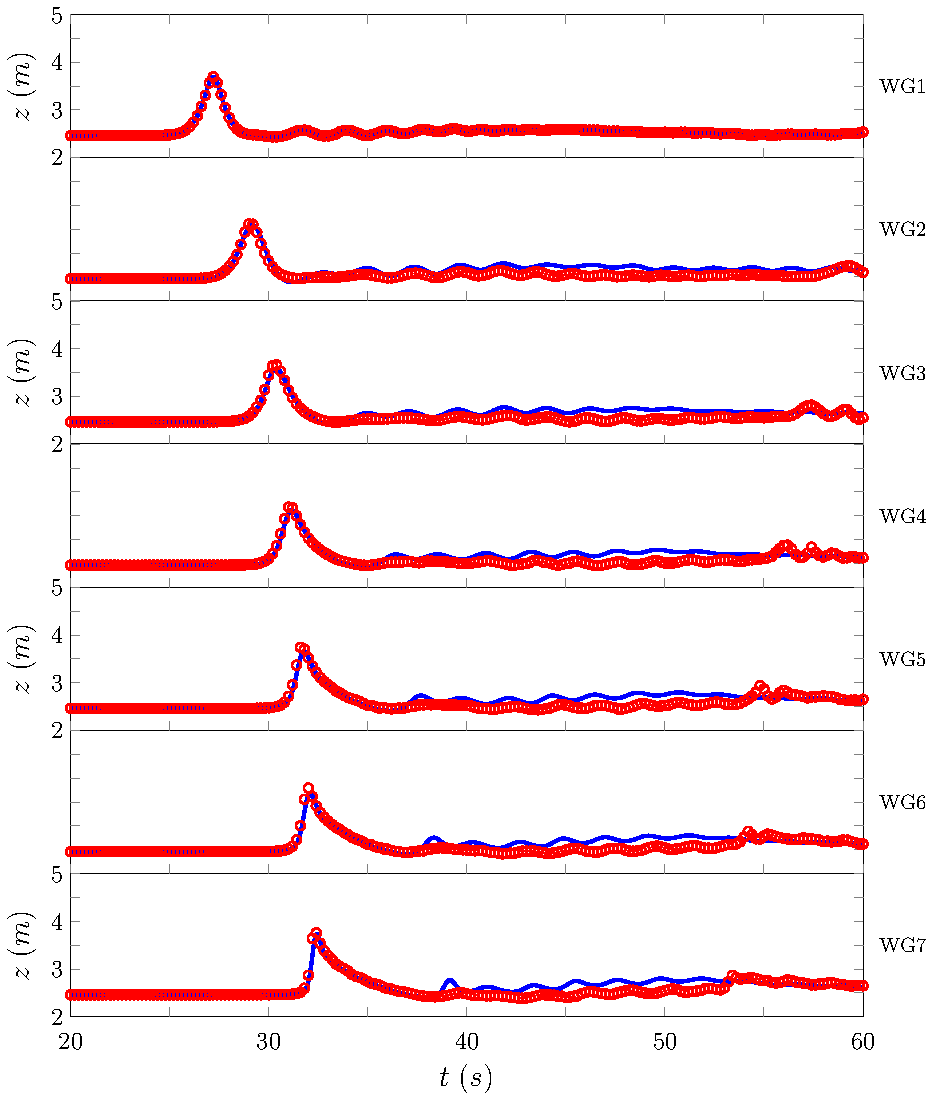
\includegraphics[width=\textwidth]{./chp6/figures/Experiment/Roeber/Trial8/FEVM/LongWGs1.pdf}
	\caption{Comparison of the experimental (\circlet{red}) and numerical ({\color{blue}\solidrule}) wave gauge data produced by $\text{FEVM}_2$ for gauges $1$ to $7$.}
	\label{fig:Roeber8WG1to7FEVM}
\end{figure}
\begin{figure}
	\centering
	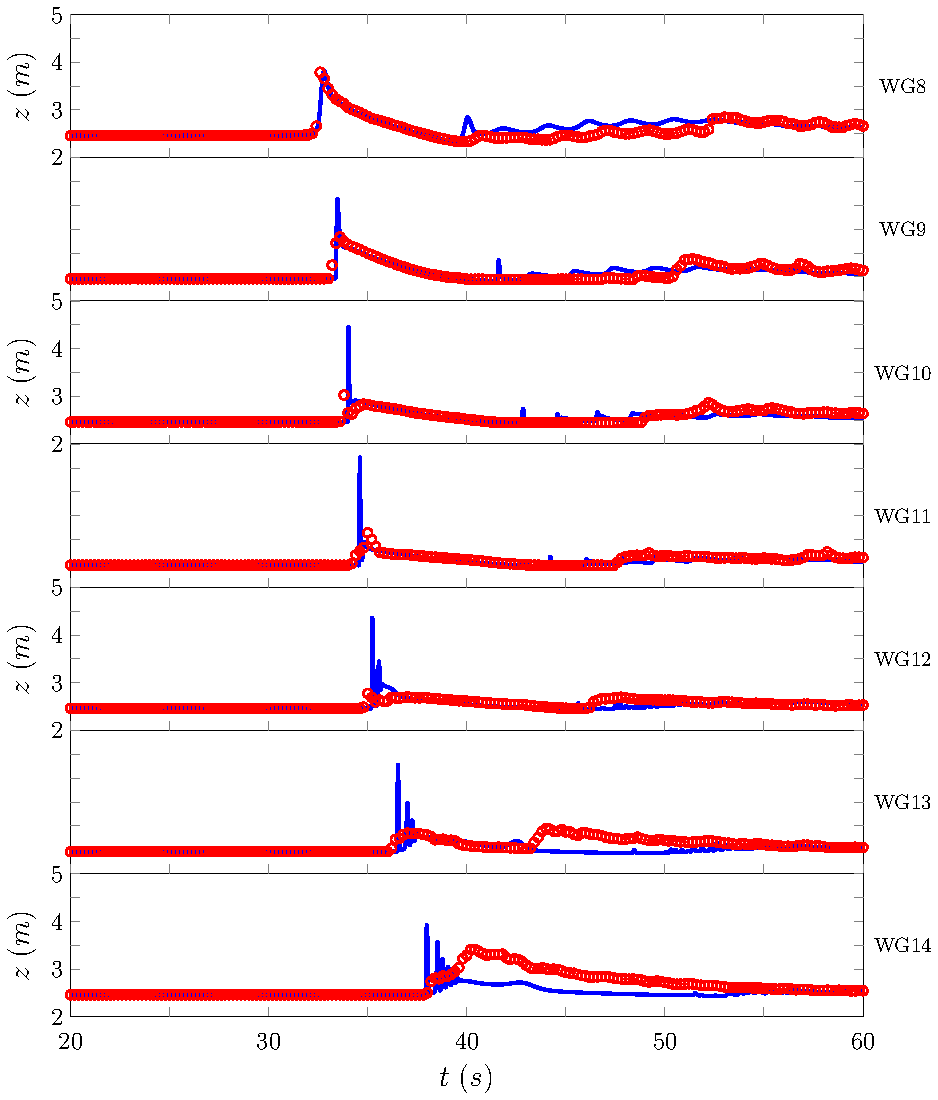
\includegraphics[width=\textwidth]{./chp6/figures/Experiment/Roeber/Trial8/FEVM/LongWGs2.pdf}
	\caption{Comparison of the experimental (\circlet{red}) and numerical ({\color{blue}\solidrule}) wave gauge data produced by $\text{FEVM}_2$ for gauges $8$ to $14$.}
	\label{fig:Roeber8WG7to14FEVM}
\end{figure}          

\begin{figure}
	\centering
	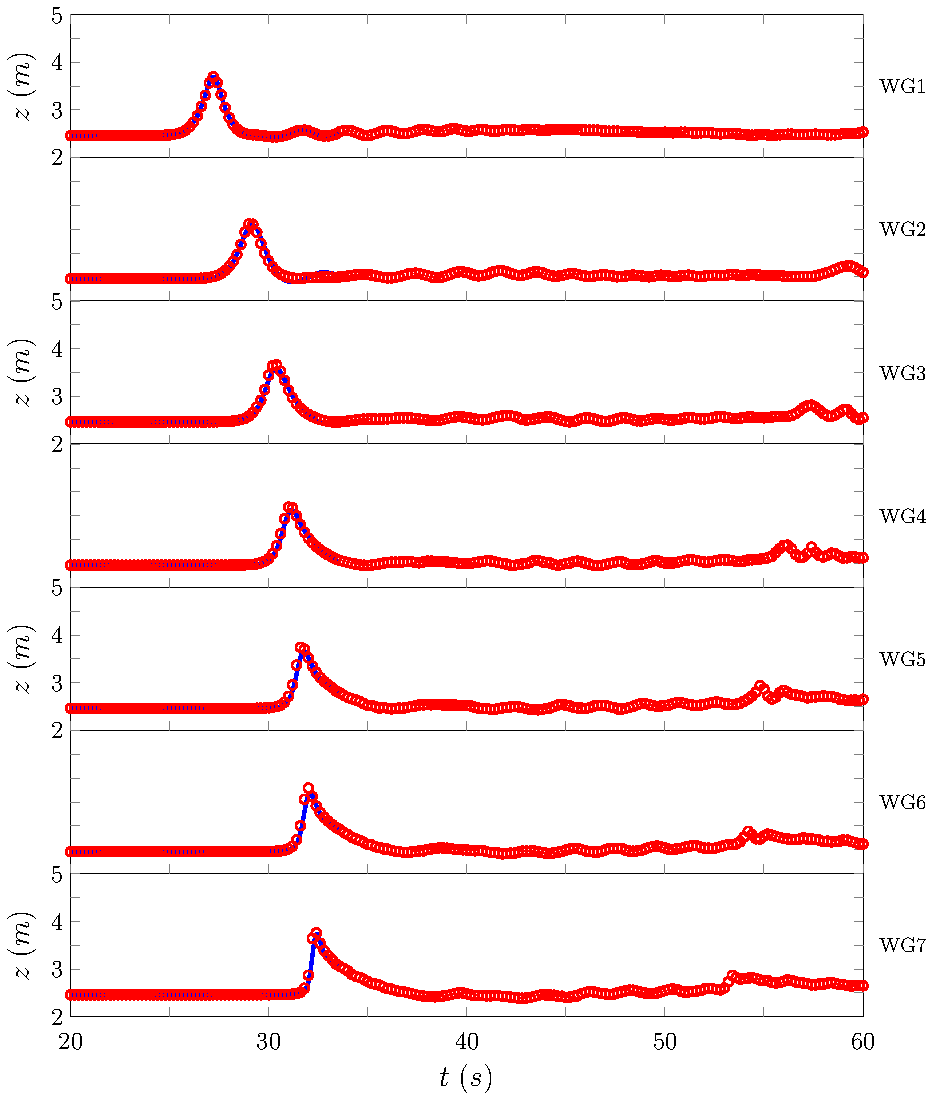
\includegraphics[width=\textwidth]{./chp6/figures/Experiment/Roeber/Trial8/FDVM/LongWGs1.pdf}
	\caption{Comparison of the experimental (\circlet{red}) and numerical ({\color{blue}\solidrule}) wave gauge data produced by $\text{FDVM}_2$ for gauges $1$ to $7$.}
	\label{fig:Roeber8WG1to7FDVM}
\end{figure}
\begin{figure}
	\centering
	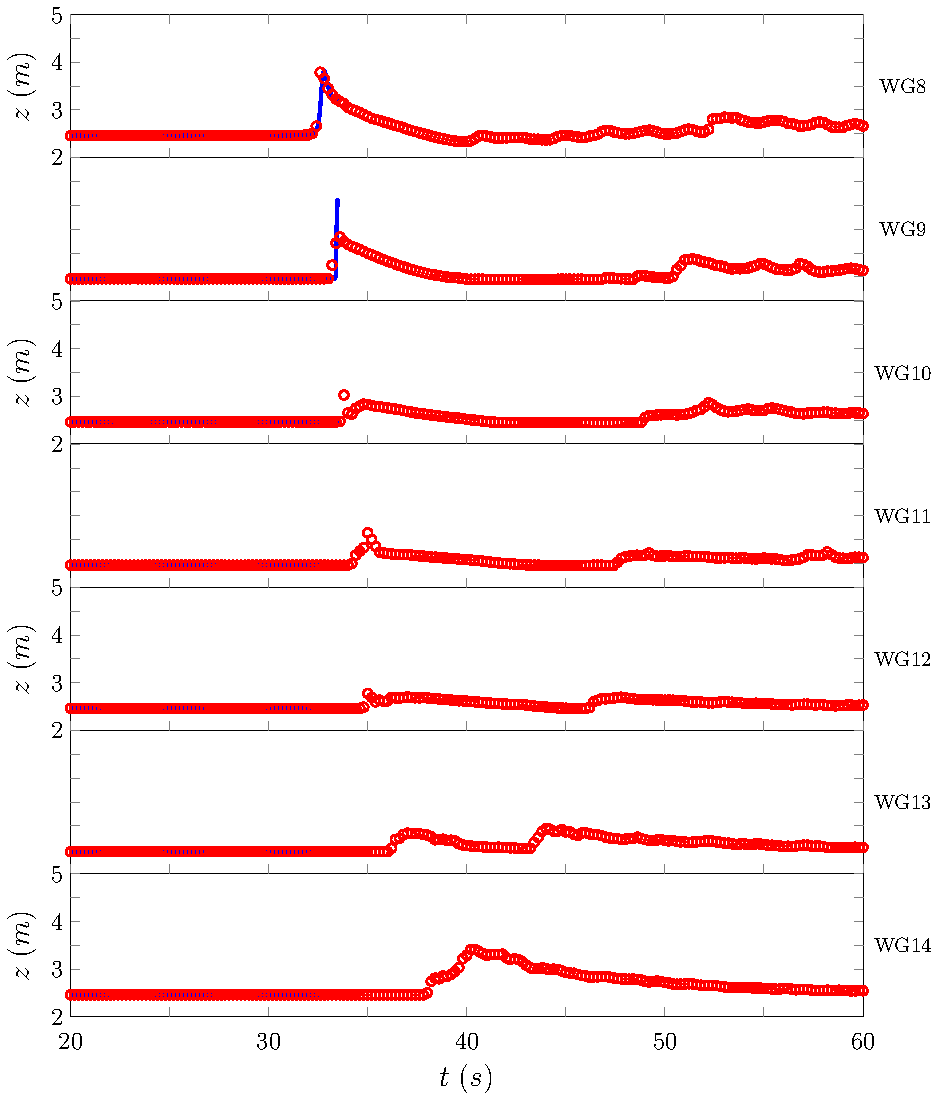
\includegraphics[width=\textwidth]{./chp6/figures/Experiment/Roeber/Trial8/FDVM/LongWGs2.pdf}
	\caption{Comparison of the experimental (\circlet{red}) and numerical ({\color{blue}\solidrule}) wave gauge data produced by $\text{FDVM}_2$ for gauges $8$ to $14$.}
	\label{fig:Roeber8WG7to14FDVM}
\end{figure} 

\section{Synolakis}
%only pointwise comparison, and H1 and C1 as wave is well defined
%comment on wave breaking number for nonlinearity




%Par 1: Experimental Design
	%nonbreaking wave shoaling

%Par 2: Explanation of Experiment and what it demonstrates
	%standard runup test

%Par 3: Numerical Experiment Design



To study the run-up of incoming waves on linear beaches a series of experiments were conducted by \citet{Synolakis-1987-523}. These experiments consisted of a number of runup events for a wide array of breaking and non-breaking waves where snapshots of the entire water surface were taken at certain times. These runs were all performed on the beach profile depicted in Figure \ref{fig:SynolakisWT}, where all the quantities are normalised \cite{Synolakis-1987-523}. To assess the computational models we recreated one of these runs, which captured the runup of a non breaking solitary wave with a nonlinearity parameter of $\epsilon = 0.0185$.

This experiment allows us to compare the inundation behaviour of our numerical methods with experimental results. For this experiment the effect of dispersion on the run-up behaviour is minimal, and there is good agreement between numerical solutions of the SWWE and this particular experiment []. Therefore, the effect of the extra dispersive terms included by the Serre equations on the inundation process is not well tested by this experiment. 

%numerical set up
The numerical experiments used the normalised quantities reported by \citet{Synolakis-1987-523} to reproduce the experiment. The spatial domain was $x' \in [-30,150]$ with a resolution of $\Delta x = 0.05$ and was run until $t' = 70$ with the CFL condition \eqref{eqn:CFLcond} satisfied by setting $\Delta t = 0.1 \Delta x$. The spatial reconstruction used the input parameter $\theta = 1.2$ and gravity was normalised to match the coordinates and so $g= 1$.
%change axis to match normalisation []


\begin{figure}
	\centering
	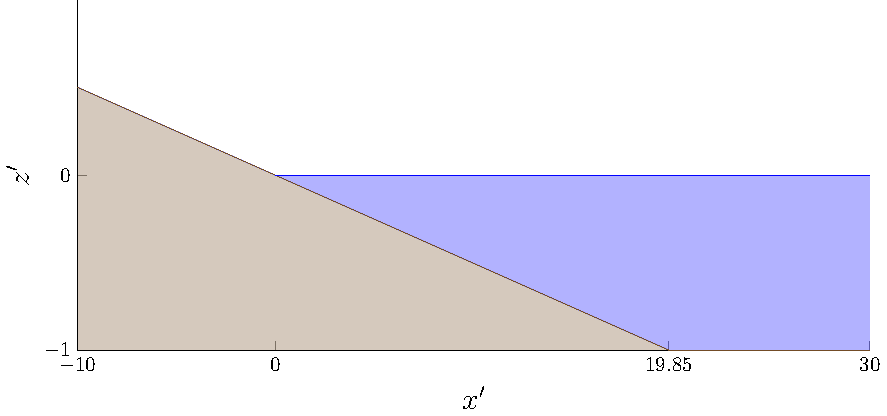
\includegraphics[width=\textwidth]{./chp6/figures/Experiment/Synolakis/WavetankArtifical.pdf}
	\caption{Diagram demonstrating the water (\squareF{blue}) and the ground  (\squareF{brown!80!black}) for the Synolakis experiments with the normalised coordinates.}
	\label{fig:SynolakisWT}
\end{figure}

\subsection{Results}

%Par 1: Figures

%Par 2: Discussion

%Par 3: Conclusion

The normalised water surface data is given at the various times in Figure \ref{fig:SynolakisFDVMNoBreak} for $\text{FDVM}_2$ and \ref{fig:SynolakisFEVMNoBreak} for $\text{FEVM}_2$. The error in conservation of the conserved quantities are given in Tables \ref{tab:ConservationSynFEVM} and \ref{tab:ConservationSynFDVM} for $\text{FEVM}_2$ and $\text{FDVM}_2$ respectively. 

Both methods reproduce the experimental results very well, replicating the incoming wave properties and the maximum runup very well. The experimental wave appears to be more skewed towards the shoreline, but this shape difference has all but disappeared as the wave begins to runup the shoreline. The only other noticeable difference is that the numerical solutions appear to run down further than the experimental results; this is because our method has no friction and so no kinetic energy is lost during runup and so the rundown phase is faster and deeper than in the experiment.

The conserved quantities are well conserved by the method; in particular the mass which even with the wetting and drying of cells has only produced a small loss of mass. The total energy of the method is also very well conserved, however the energy appears to have slightly increased in the method during the run-up process and the desingularisation transformation used to handle the dry beds. Because the end of the experiment occurs as the wave runs down the wave has been reflected and so its total $G$ and momentum have switched signs, accounting for this the error in momentum and $G$ is quite small but much larger than the other values, this is due to our inability to accurately take account of the source term in their equations as kinetic energy is transferred into gravitational potential energy over the dry bed. 

The results for both $\text{FEVM}_2$ and $\text{FDVM}_2$ are identical in these Figures as these grids are quite fine and so these figures represent a good approximation to the true solution of the Serre equations. These numerical solutions demonstrate good agreement with experimental results and display the capability of the method for the inundation of non-breaking waves.

\begin{figure}
	\centering
	\begin{subfigure}{0.5\textwidth}
		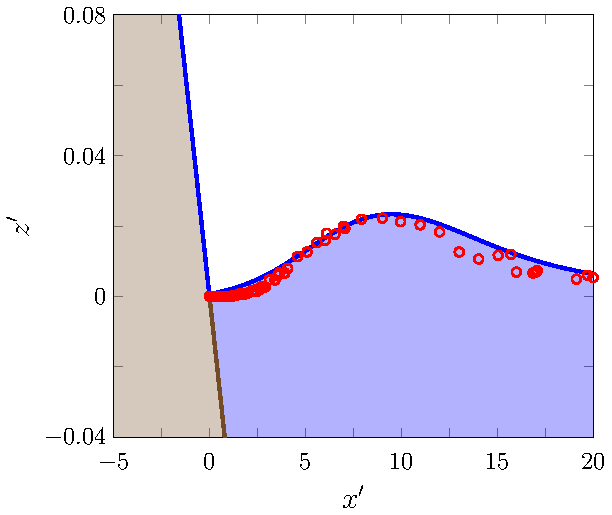
\includegraphics[width=\textwidth]{./chp6/figures/Experiment/Synolakis/H0p0185/FEVM/30s.pdf}
		\subcaption{$t=30s$}
	\end{subfigure}%
	\begin{subfigure}{0.5\textwidth}
		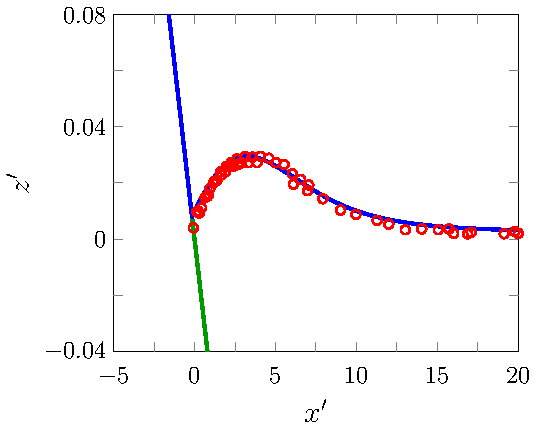
\includegraphics[width=\textwidth]{./chp6/figures/Experiment/Synolakis/H0p0185/FEVM/40s.pdf}
		\subcaption{$t=40s$}
	\end{subfigure}
	\begin{subfigure}{0.5\textwidth}
		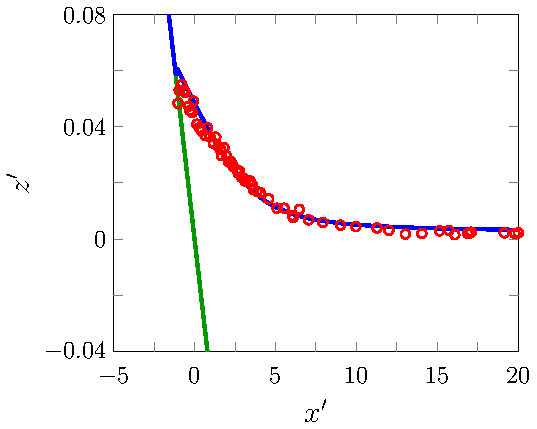
\includegraphics[width=\textwidth]{./chp6/figures/Experiment/Synolakis/H0p0185/FEVM/50s.pdf}
		\subcaption{$t=50s$}
	\end{subfigure}%
	\begin{subfigure}{0.5\textwidth}
		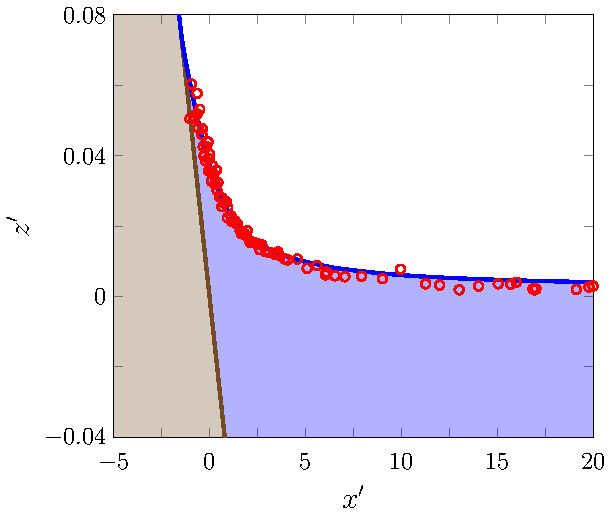
\includegraphics[width=\textwidth]{./chp6/figures/Experiment/Synolakis/H0p0185/FEVM/60s.pdf}
		\subcaption{$t=60s$}
			\end{subfigure}
	\begin{subfigure}{0.5\textwidth}
		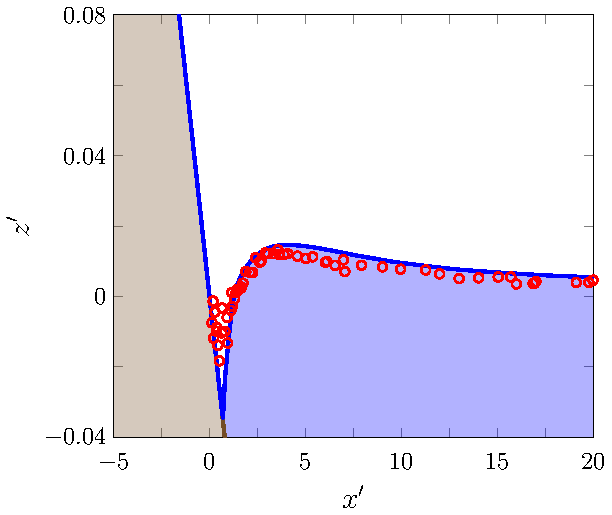
\includegraphics[width=\textwidth]{./chp6/figures/Experiment/Synolakis/H0p0185/FEVM/70s.pdf}
		\subcaption{$t=70s$}
	\end{subfigure}
	\caption{A comparison of the water surface profiles for the experiment (\circlet{red}) and the numerical solution ({\color{blue}\solidrule}) produced by $\text{FEVM}_2$ at various times.}
	\label{fig:SynolakisFEVMNoBreak}
\end{figure}

\begin{figure}
	\centering
	\begin{subfigure}{0.5\textwidth}
		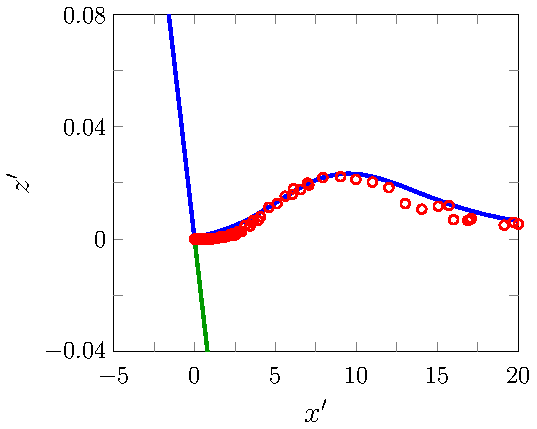
\includegraphics[width=\textwidth]{./chp6/figures/Experiment/Synolakis/H0p0185/FDVM/30s.pdf}
		\subcaption{$t=30s$}
	\end{subfigure}%
	\begin{subfigure}{0.5\textwidth}
		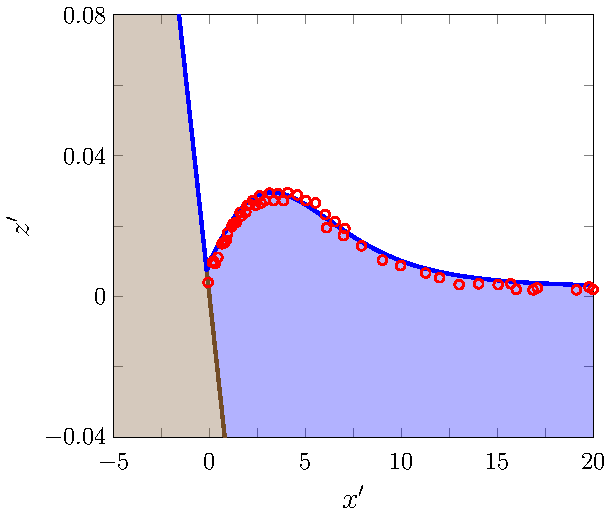
\includegraphics[width=\textwidth]{./chp6/figures/Experiment/Synolakis/H0p0185/FDVM/40s.pdf}
		\subcaption{$t=40s$}
	\end{subfigure}
	\begin{subfigure}{0.5\textwidth}
		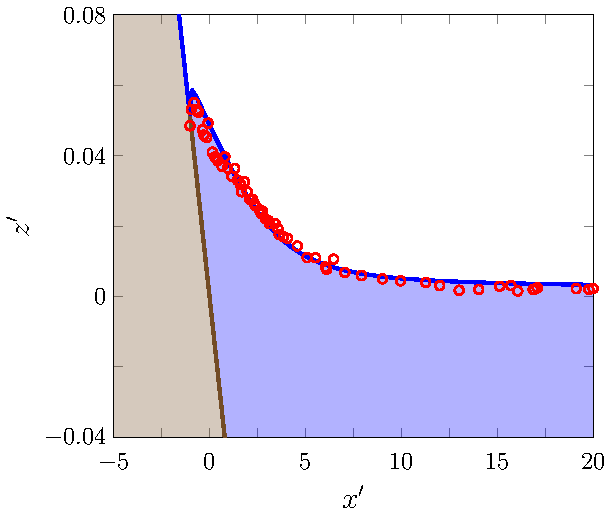
\includegraphics[width=\textwidth]{./chp6/figures/Experiment/Synolakis/H0p0185/FDVM/50s.pdf}
		\subcaption{$t=50s$}
	\end{subfigure}%
	\begin{subfigure}{0.5\textwidth}
		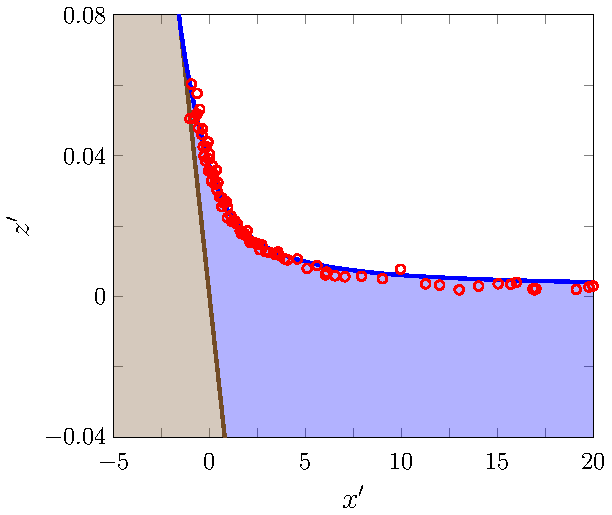
\includegraphics[width=\textwidth]{./chp6/figures/Experiment/Synolakis/H0p0185/FDVM/60s.pdf}
		\subcaption{$t=60s$}
	\end{subfigure}
	\begin{subfigure}{0.5\textwidth}
		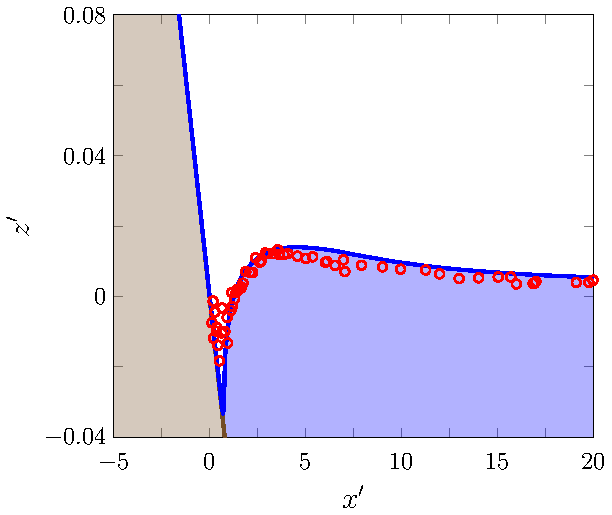
\includegraphics[width=\textwidth]{./chp6/figures/Experiment/Synolakis/H0p0185/FDVM/70s.pdf}
		\subcaption{$t=70s$}
	\end{subfigure}
	\caption{A comparison of the water surface profiles for the experiment (\circlet{red}) and the numerical solution ({\color{blue}\solidrule}) produced by $\text{FDVM}_2$ at various times.}
	\label{fig:SynolakisFDVMNoBreak}
\end{figure}

%Negative energy
\begin{table}
	\centering
	\begin{tabular}{l  c  c c}
		Quantity& $\mathcal{C}^*\left(\vecn{q}^0\right)$ & $\mathcal{C}^*\left(\vecn{q}^*\right)$ & $\mathcal{C}^*_1\left(\vecn{q}^0,\vecn{q}^*\right)$ \\
		\hline &&& \\
		Mass & $140.41696534392645$ & $140.416965345$ & $-7.65\times 10^{-12}$\\
		Momentum & $-0.31905013851476244$ & $0.320317183357$ & $0.0040$\\
		$G$ & $-0.31907372312696913$ & $0.320448924368$ & $0.0043$\\
		Energy & $-68.38995818739492$ & $-68.3914362911 $ & $2.16 \times 10^{-5}$ \\
	\end{tabular}
	\caption{Total amounts and error in conservation for all quantities for $\text{FEVM}_2$ numerical solution of the runup experiment.}
	\label{tab:ConservationSynFEVM}
\end{table}

\begin{table}
	\centering
	\begin{tabular}{l  c  c c}
		Quantity& $\mathcal{C}^*\left(\vecn{q}^0\right)$ & $\mathcal{C}^*\left(\vecn{q}^*\right)$ & $\mathcal{C}^*_1\left(\vecn{q}^0,\vecn{q}^*\right)$ \\
		\hline &&& \\
		Mass & $140.41696534392645$ & $140.416949821$ & $1.11\times 10^{-7}$\\
		Momentum & $-0.31905013851476244$ & $0.319579326905$ & $0.0017$\\
		$G$ & $-0.31907372312696913$ & $0.320668702008$ & $0.0050$\\
		Energy & $-68.38995818739492$ & $-68.3914356777 $ & $2.16 \times 10^{-5}$ \\
	\end{tabular}
	\caption{Total amounts and error in conservation for all quantities for $\text{FDVM}_2$ numerical solution of the runup experiment.}
	\label{tab:ConservationSynFDVM}
\end{table}

